\nonstopmode

\documentclass
[
    a4paper,
    twoside,
    12pt,
]
{report}
\usepackage[utf8]{inputenc}
\renewcommand{\familydefault}{\rmdefault}
\usepackage[a4paper, left=3.19cm, right=3.19cm, top=2.54cm, bottom=2.54cm]{geometry}
\usepackage[american]{babel}
\usepackage{csquotes}
\usepackage{float}
\usepackage{enumerate}
\usepackage[bottom]{footmisc}
\usepackage{array}
\usepackage{ntheorem}
\usepackage{parskip}
\usepackage[right]{eurosym}
\usepackage{xcolor}
\usepackage[hyphens]{url}
\usepackage{makeidx}
\usepackage{multicol}
\usepackage{theorem}
\usepackage{amsmath}
\usepackage{listings}
\usepackage{graphicx}
\usepackage{subcaption}
\usepackage{pgfplots}
\pgfplotsset{compat=1.5}
\usepackage{csvsimple}
\usepackage{fancyhdr}
\usepackage{colortbl}
\usepackage{bchart}
\usepackage[hidelinks]{hyperref}
\usepackage{setspace}
\usepackage{mathptmx}
%\usepackage{showframe}
\pagestyle{plain}
\rhead{\thepage}
\sloppy

\usepackage[
backend=biber,
style=apa,
citestyle=authoryear
]{biblatex}

\addbibresource{references.bib}
\DeclareLanguageMapping{american}{american-apa}
\def\sectionautorefname{Section}

%\setlength{\unitlength}{1cm}
%\setlength{\oddsidemargin}{0.3cm}
%\setlength{\evensidemargin}{0.3cm}
%\setlength{\textwidth}{15.5cm}
%\setlength{\topmargin}{-1.2cm}
%\setlength{\textheight}{24.7cm}
%\columnsep 0.5cm

%\title{Seminararbeit}
\selectcolormodel{cmyk}{

\newcommand{\Arbeitstitel}
	{
  	Success factors of video game consoles
	}
\newcommand{\Autor}
	{
		Dipl.-Ing. (FH) Lars Bartschat
	}

\newcommand{\MatrikelNr}
	{
		WBPA140000250
	}

\newcommand{\EmailAdresse}
	{
		bartschat@mailbox.org
	}
\newcommand{\Arbeitsart}
	{
		Seminar Paper
	}
\newcommand{\Studiengang}
	{
		Marketing Executive Program
	}
\newcommand{\Hochschule}
	{
		University of Münster
	}
\newcommand{\Lehrstuhl}
	{
		Department of Marketing and Media Research
	}
\newcommand{\Themensteller}
	{
		Prof. Dr. T. Hennig-Thurau
	}
\newcommand{\Betreuer}
	{
		M. Sc. R. Behrens
	}
\newcommand{\Ausgabedatum}
	{
		17.10.2016
	}
\newcommand{\Abgabedatum}
	{
		28.11.2016
	}
\newcommand{\Ort}
	{
		Münster}
			
		
\newcommand{\link}[1]{\ref{#1} (S. \pageref{#1})}
\begin{document}

\begin{titlepage}
    \vspace*{1.0cm}
    \begin{center}
        \begin{Large}
        \textbf{An investigation of accent conversion for non-native and native varieties of English} \\
        \end{Large}
        \vspace*{1.0cm}
        \textit{Kenny W. Lino} \\
        \vspace*{1.5cm}
        M.Sc. Dissertation \\
        \vspace*{0.5cm}
        \begin{figure}[H]
        \centering
        
\includegraphics[scale=0.15]{img/UM-coat-of-arms.png}
    	\end{figure}
       \vspace*{1.0cm}
       Department of Intelligent Computer Systems \\
       Faculty of Information and Communication Technology \\
       University of Malta \\
       2018 \\
       
       \vspace*{2.0cm}
	   Supervisors: \\
       Claudia Borg, Department of Artificial Intelligence, University of Malta \\
       Andrea DeMarco, Institute of Space Sciences and Astronomy, University of Malta \\
       Eva Navas, Department of Communications Engineering, University of the Basque Country \\
       
       \vspace*{4.0cm}
       Submitted in partial fulfilment of the requirements for the Degree of \\
       European Master of Science in Human Language Science and Technology
    \end{center}



\end{titlepage}

\onehalfspacing
\pagenumbering{Roman}

\cleardoublepage

\begin{center}
  M.Sc (HLST) \\
  \uppercase{\textbf{Faculty of Information and \\
  Communication Technology \\ University of Malta \\ }}
  \vspace*{0.5cm}
  Declaration \\
\end{center}
  \vspace*{1.5cm}
        Plagiarism is defined as "the unacknowledged use, as one's own work, of work of another person, whether or not such work has been published" (Regulations Governing Conduct at Examinations, 1997, Regulation 1 (viii), University of Malta). \\

I, the undersigned, declare that the Master's dissertation submitted is my own work, except where acknowledged and referenced. \\

I understand that the penalties for making a false declaration may include, but are not limited to, loss of marks; cancellation of examination results; enforced suspension of studies; or expulsion from the degree programme. \\
       
       \vspace*{1.5cm}
	     Student Name: Kenny W. Lino \\
       Course Code: CSA5310 HLST Dissertation \\
       Title of work: An investigation of accent conversion for non-native and native varieties of English \\

       \vspace*{1.0cm}
       Signature of Student: \\

       \vspace*{1.0cm}
       Date:

\newpage
\section*{Abstract}
\addcontentsline{toc}{section}{Abstract}

With the emergence of the use of technology in language learning through
tools like Rosetta Stone and Duolingo, learners have slowly been given
more autonomy of their language learning projection. Although these
tools have allowed learners to tailor their learning to their own
liking, there is a gap between the available resources to assist those
that would like to improve their pronunciation. Previous research in the
intersection of language learning and speech technology has made efforts
to develop pronunciation training systems to address this problem, but
the systems themselves tend to have gaps due to the lack of appropriate
support for the users, especially in appropriately identifying errors
and providing sufficient feedback to help them correct their errors.

Some researchers have purported that alongside other forms of feedback
such as a visual articulatory representation, a voice conversion system
could serve as a potential feedback mechanism by helping learners
understand what their voice could sound like given the appropriate
changes. However, like pronunciation training systems, voice conversion
systems also faced many limitations due to the complex interaction of
various features which made them unrenderable as useful tools. With that
said, recent advances in speech technology using methods such as
i-vectors and deep neural networks have become increasingly successful
in achieving better accuracy and quality in a variety of tasks, allowing
for the potential to return and address these said gaps in performance
for voice conversion.

This dissertation investigates these advancements in applying i-vectors
and deep neural networks to develop an accent conversion system (a
modified voice conversion system) that could potentially serve as a
feedback mechanism as a part of a larger computer-based pronunciation
training system. I compare this methodology against baselines using more
traditional features and conversion processes following the work of
Aryal and Gutierrez (2014) among their other works, and evaluate using
the responses of participants in a perceptual study. I conclude with a
discussion of the current work and highlight some potential directions
for future direction.
\cleardoublepage
\tableofcontents
\addcontentsline{toc}{section}{Contents}
\clearpage
\listoffigures
\addcontentsline{toc}{section}{List of Figures}

\section*{List of Abbreviations}
\addcontentsline{toc}{section}{List of Abbreviations}
\begin{tabular}{ll}
    \colorbox{magenta}{Keep this updated} \\
    CAPT    & Computer Assisted Pronunciation Training \\
    CP      & Critical Period \\
    GMM     & Gaussian Mixture Model \\
    L1/L2    & First and second language \\
    LSTM & Long-short term memory \\
    MFCC & Mel-frequency cepstrum coefficient \\ 
    TTS   & Text-to-speech \\
    
\end{tabular}

\clearpage
\cleardoublepage
\pagenumbering{arabic}
\setcounter{page}{1}

\chapter{Introduction}

\colorbox{magenta}{[Cite robustness of Alexa, Siri, Google Translate and viral videos]}

While technology has flourished and led to a number of new
state-of-the-art systems such as improvements in commercial speech
recognition and machine translation, it can be argued that these
benefits have not reached all potential users and uses to the same
extent. For example, many commercial systems like Google Translate,
Siri, Alexa, etc. have grown in the number of languages they have
available, but when considering the robustness of these systems across
languages, it is often evident that the systems function much better
with languages that have more speakers across the globe such as English
or Spanish. In some cases such as with newer products, a user's native
language might not yet even be available, which can cause them to
relegate to English.

These systems are also often better equipped to work with specific
language varieties, which are often considered to be the `standard' or
more common variety of that language. In the context of speech
recognition systems, this means that this could cause potential
challenges for speakers of other varieties-- or \emph{accents}, whether
it be another native but `non-standard' accent or a non-native accent.
This issue can be observed in various viral videos, such as an Italian
grandmother who is trying to activate a Google Home device by saying,
``Okay Google!'' or another video where a woman is trying to get her
Amazon Alexa device to play a song called ``Something's Cooking in My
Kitchen by Dana''. In both cases, both women have issues with their
devices properly understanding them likely because they speak English
with an accent that the systems are not (well-)trained on.

Yet when it comes to accents, teaching them can be as equally difficult
as trying to have them recognized by speech recognition systems. This
extends into language teaching and learning as well, where learners of a
second language often have trouble acquiring proper pronunciation. In
fact, pronunciation has been a large standing challenge in language
learning due to its complex nature. Unlike grammar and vocabulary, which
many language learners acquire without issue, pronunciation can be
challenging to both learn and teach due to the lack of clarity on how to
teach it. This is because pronunciation involves a number of nuanced
characteristics, including stress, rhythm, vowels, and consonants, which
can vary just small enough for one language or accent to draw a
distinction, while others conflate them.

In order to address these issues in speech recognition and language
learning, researchers have investigated variation solutions. Linguists
focused on language learning and phonetics have examined the underlying
causes of what creates obstacles in learning an accent, with some
concluding that native-like accents are nearly unobtainable after a
certain age threshold. Regardless of this conclusion, some researchers
have turned to language technology to develop potential pronunciation
training systems with the hopes of any possible accent reduction.
Earlier studies using some of these pronunciation training systems have
shown that while they have the potential, many of them suffer from the
lack of appropriate feedback that the user can understand. Thus, some
researchers have pointed to the potential use of accent conversion as a
mode of feedback as it has been hypothesized that hearing one's voice
pronounce something with the desired accent is better feedback as
compared to a point system or spectrograms, which require specialized
training to interpret.

Accent conversion has also been proposed as a potential solution to
challenges in speech recognition. Because speech recognition is often
trained on large amounts of speech data, it can be unrealistic to
attempt to collect sufficient speech data for the endless possible
varieties or accents that exist for a single language. Instead,
researchers have pointed to accent conversion as a possible way to adapt
current available systems to more speakers, with the idea that accent
conversion could change the accent of a speaker into sounding more like
an accent the speech recognition system can better recognize without
training it on a large amount of data. This can be viewed similarly to
other natural language processing tasks, such as text classification or
part-of-speech tagging of varying genres such as formal news text
vs.~informal blogs or tweets, where currently available systems have
been adapted to perform better on more genres instead of creating
specialized systems for each genre type.

\hypertarget{what-is-an-accent}{%
\section{What is an ``accent''?}\label{what-is-an-accent}}

Before continuing on, it is best to define what accent is, especially in
the context of this work. Accents consist of a number of features,
including the vowels and consonants, the stress, rhythm, intonation, and
even pauses that a speaker uses. The variation in these features
contribute to what many known as \emph{accent}, or variations in
pronunciation across speakers based on location, ethnicities, social
classes, native languages, etc. \colorbox{magenta}{[Cite this]} Accents
can be considered to be a part of dialects, where users of the same
language may have variations beyond pronunciation, such as usage in
vocabulary or grammar. The line may often be blurred in everyday
discussions and even in academic analyses as accent and dialect (as well
as language) could be considered to be on a continuum, but for the sake
of simplicity, I consider \emph{accent} to be variations in
pronunciation in this work.

\hypertarget{research-questions}{%
\section{Research Questions}\label{research-questions}}

In this thesis, I focus on investigating the following questions:

\begin{itemize}
\item
  How can we leverage accent conversion to change the accent of a
  \emph{non-native speaker} into sounding more like a \emph{native
  speaker}? (e.g.~converting the accent of a native Spanish speaker to
  sound more like a US English speaker)
\item
  How can we leverage accent conversion to change the accent of two
  \emph{native speakers} of English who speak two distinct varieties?
  (e.g.~converting the accent of a Scottish speaker to sound more like a
  Standard Southern English speaker)
\item
  To what extent can we maintain the voice characteristics of the
  selected speakers, or \emph{the identity} when converting their
  accents? (e.g.~Can we convert the accent of a speaker and make sure it
  still sounds like the same person?)
\end{itemize}

\hypertarget{thesis-overview}{%
\section{Thesis Overview}\label{thesis-overview}}

The overview of the thesis is as follows:

In \textbf{Chapter 2}, I give a proper definition of voice conversion
and accent conversion, and a high level overview of some technical
details needed to better understand the current work.

In \textbf{Chapter 3}, I present the motivation for creating an accent
converison system by discussing previous findings in second language
acquisition research especially in relation to speech. I then cover
previous work in voice and accent conversion to frame the advances and
shortcomings of previously developed systems.

In \textbf{Chapter 4}, the design and methodology of the experiments are
presented alongside the appropriate tools utilized to conduct each one.

In \textbf{Chapter 5}, the results of the experiments previously
described are presented along with some short discussion and conclusions
drawn from the results.

In \textbf{Chapter 6}, the thesis is concluded with a reflection on the
work presented along with some appropriate suggestions for future work.
\cleardoublepage

\chapter{Background}

Before delving into previous literature and their relevance to this work
and the fields of NLP and language learning as a whole, I detail both
voice conversion and accent conversion in order to help better
distinguish them. I also go over some common speech technology concepts
typically used in these systems at a high level in order to make the
current work more accessible to those unfamiliar with the area. Further
reference is also provided for those interested in the more technical
aspects and formalisms.

\hypertarget{voice-conversion}{%
\section{Voice conversion}\label{voice-conversion}}

To properly frame voice conversion, we take a look at
\textcite{mohammadi2017} who present a recent overview of the subfield.
Following a definition setforth by the authors, voice conversion refers
to the transformation of a speech signal of a \emph{source speaker} to
make it sound as if it were uttered by a \emph{target speaker} in any
chosen fashion with the utterance still being intact. Some of these
changes can include changes in emotion, accent, or phonation
(whispered/murmured speech). there have been a number of proposed uses
for VC, including the transformation of speaker identity (perhaps for
voice dubbing), personalized TTS systems, and against biometric voice
authentication systems.

Voice conversion often involves a large number of processes, one of
which includes deciding the appropriate type of data. To start, one must
decide whether to have parallel or non-parallel speech data. Parallel
speech data refers to speech data that has source and reference speakers
that say the same utterance, so only the speaker-specific information is
different, while non-parallel data would indicate datasets where the
utterances are not the same, and thus entail further processes to create
a target waveform. Even though parallel corpora are more desirable as it
reduces the footprint necessary for conversion, parallel corpora are
often curated for specific purposes and are not available in most cases.
Because of its simplicity, in some cases, researchers have tested making
a psuedo-parallel corpus using acoustic clustering when working with
non-parallel data \parencite{lorenzo-trueba2018, sundermann2006}.

Other aspects that need to be considered as discussed by
\textcite{mohammadi2017} include whether the data is
\emph{text-dependent} or \emph{text-independent}. Text-dependent corpora
indicate that the data has word or phonetic transcription, which can
ease the alignment process during training, while systems using
text-independent data would need to find similar speech segments, using
a method like acoustic clustering before training. Finally, one minor
aspect that is not considered often is the languages of the source
speaker and target speaker. Although many systems tend to focus on voice
conversion between two native speakers of the same language, systems
that aim to convert between two speakers speaking in different languages
would have to be wary of potential mapping issues between sounds. This
is especially important to consider in terms of accent conversion, which
will be discussed in the following section.

Aside from considering these aspects of the corpora, the type of
features extracted from the waveforms heavily impact the quality of the
conversions. In investigating the most salient features of speaker
individuality, previous researchers have concluded that the average
spectrum, formants, and average pitch level are the most relevant.
Following these conclusions, most VC systems focus on converting these
features, and often work at the frame-level (windows of
\begin{math}\sim\end{math}20ms), with the assumption that the frame
represents a stationary sound. From these frames, there are a number of
common local features that are extracted to represent the signal. These
include the spectral envelope, cepstrum, line spectral frequencies (LSF)
and the aforementioned formants. On top of these local frame-based
features, contextual features can be considered as well as the local
features alone are often limited in what they can model. These
contextual features can be as simple as adding delta and delta delta
features, although methods such as something known as event-based
encodings have been tested as well. With event-based encodings, a
sequence of local features are separated into different event targets
and transitions to model an utterance. However, this method faces the
challenge of properly defining events within the sequence. Thus,
although many algorithms and methods exist to model a signal, most
systems focus on working with mel-frequency cepstrum coefficents (MFCCs)
and deltas/double deltas, as they are very standard in most speech
synthesis and recogntion systems in general. The extraction process of
MFCCs and deltas/double deltas are described in further detail in
\autoref{technical-background}.

After the chosen features are extracted, the features between the source
speaker and target speaker have to be matched to prepare them for
conversion. In parallel conversion, this means that each sound in an
utterance has to be mapped between the speakers, which can be done
manually but more often is done using an algorithm such as dynamic time
warping (DTW). Although this is usually an effective algorithm to find
the best alignment, there can be issues in aligning the sounds as it
assumes that the same phonemes of the speakers have similar features
\parencite{mohammadi2017}. This can be improved upon by adding phonetic
transcription, or using methods such as forced alignment, but these
methods may also have other limitations.

With non-parallel voice conversion, the alignment process becomes more
complex as utterances from the source and target speakers have to be
broken down into individual phonemes, and then the desired sounds must
somehow be collected and synthesized to produce the converted speech.
This can be done using methods like unit-selection text-to-speech (TTS),
but this requires a large amount of annotated training data. Algorithms
such as INCA can be used in addition to work without annotation by
iteratively searching for the best frame pairs. Further information on
the various alignment methods are detailed within
\textcite{mohammadi2017}.

When the best frames between the source and target speakers are finally
matched, a method has be to chosen to map the relationship between the
frames. This has traditionally been done by using Gaussian Mixture
Models, although neural networks have also become prevalent as well as
they become ubiquitous throughout computational modeling. A detailed but
accessible explanation of these algorithms and how they function is
provided in \autoref{technical-background}.

A visual representation that summarizes the voice conversion process can
be seen in \autoref{fig:vc-flowchart}, courtesy of
\textcite{mohammadi2017}.

\begin{figure}[H]
\centering
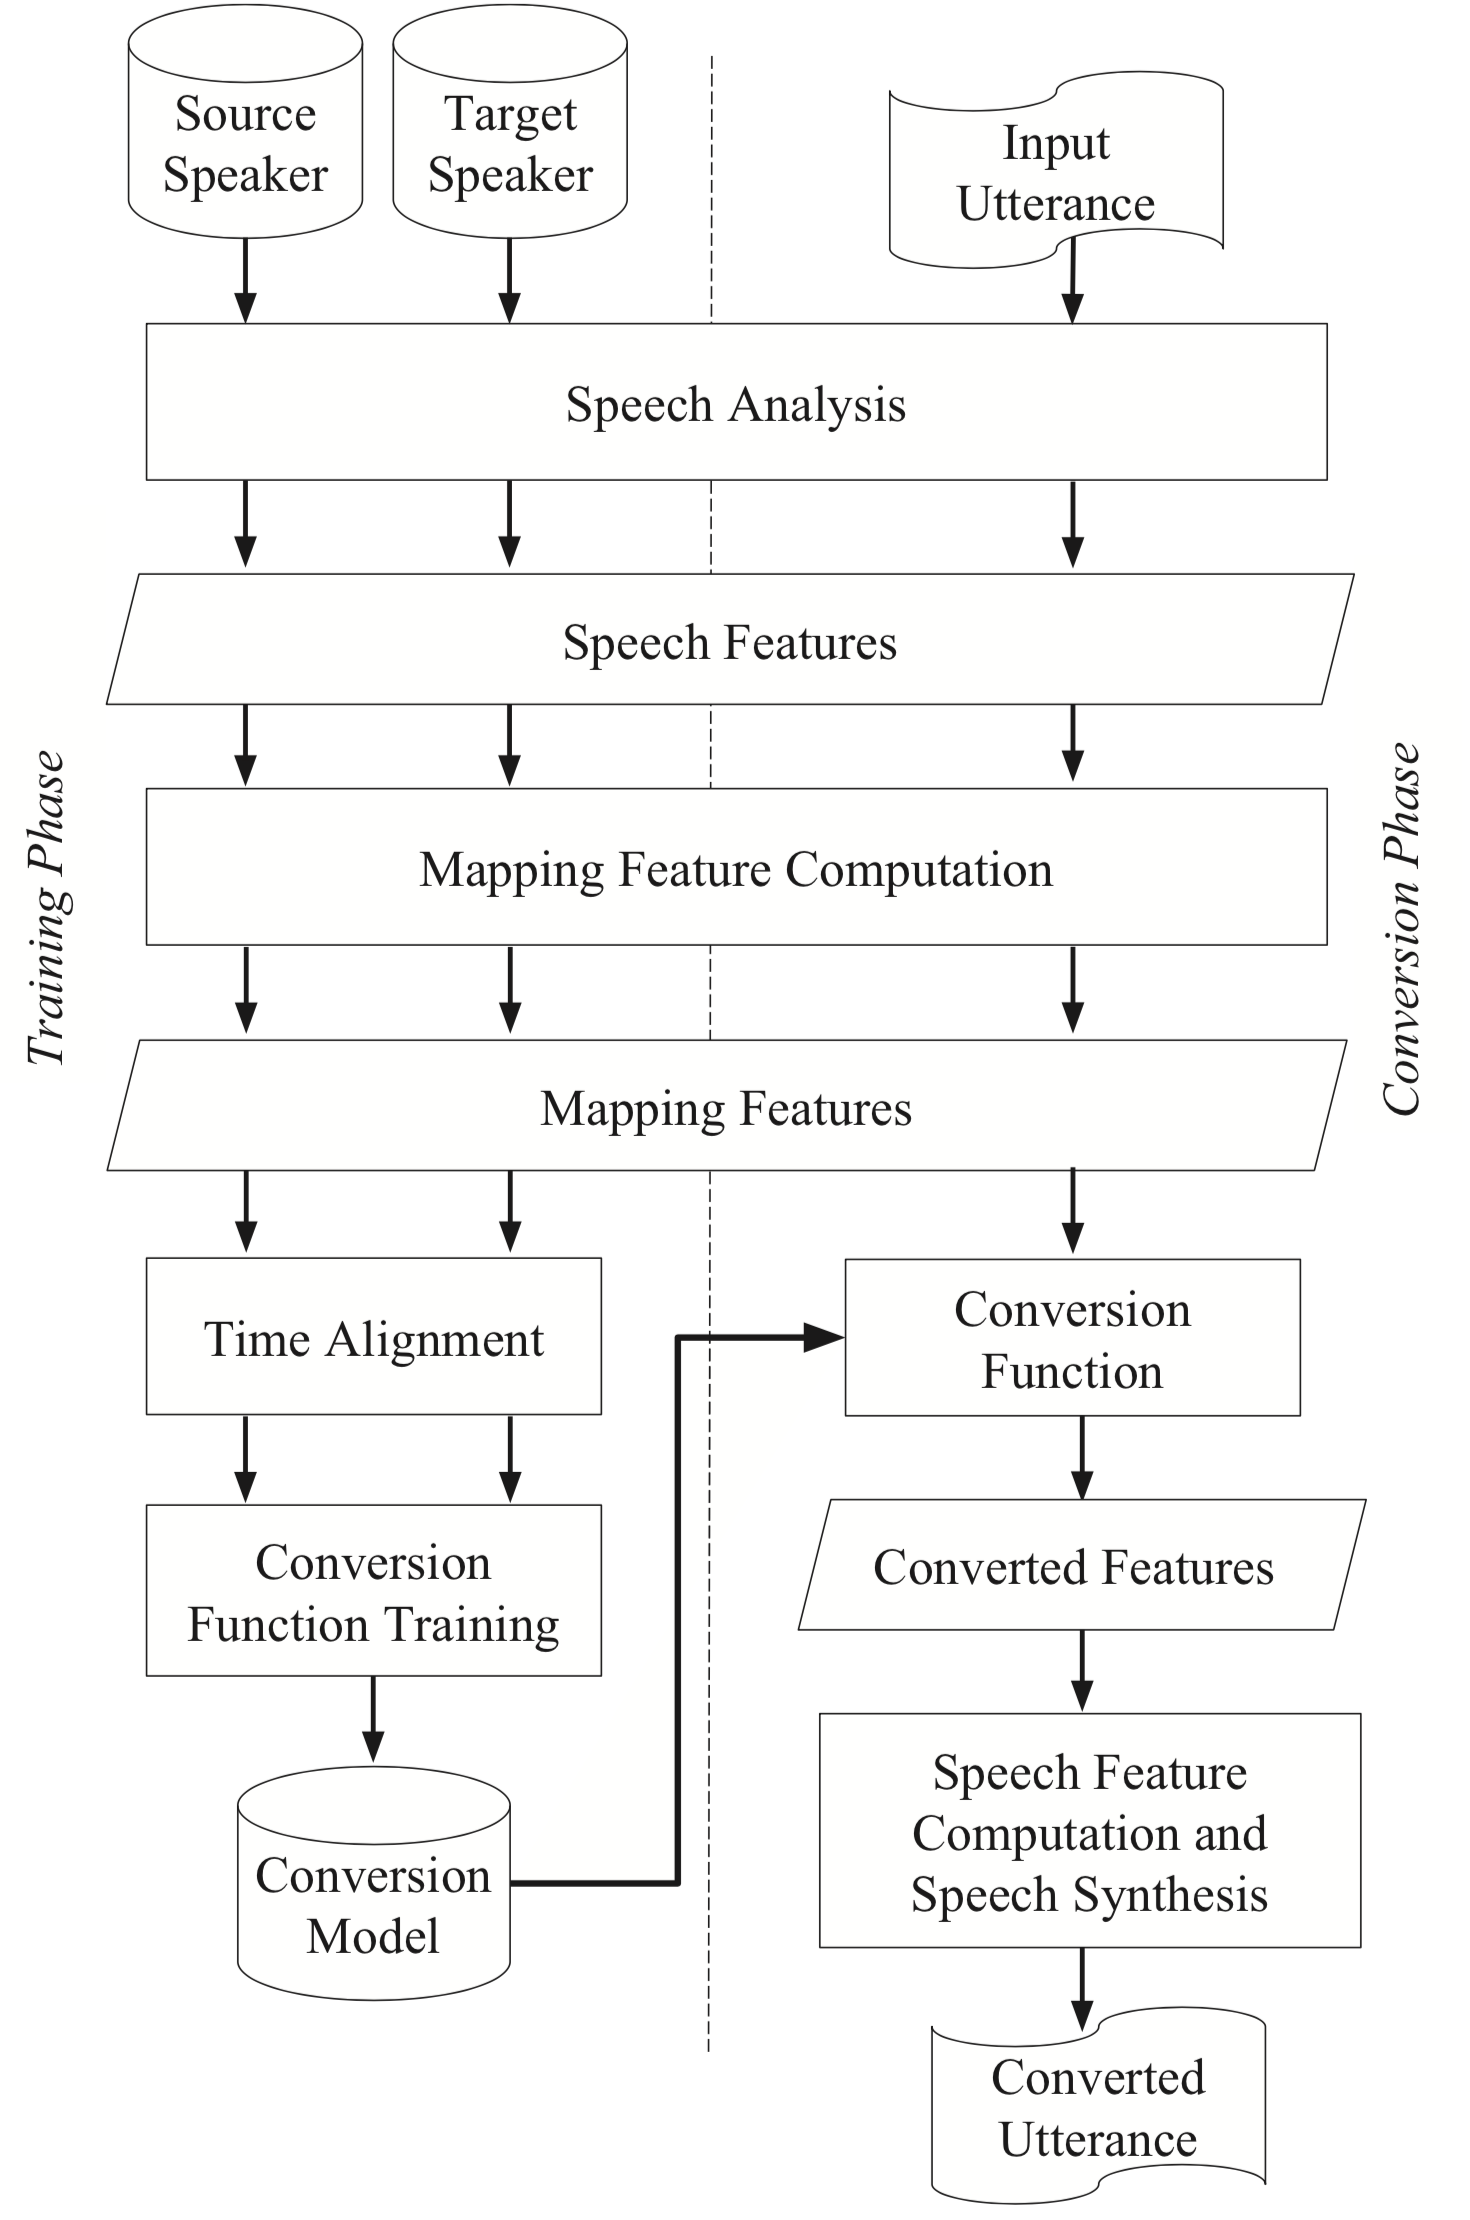
\includegraphics[scale=0.25]{img/vc-flowchart.png}
\caption{The training and conversion processes of a typical VC system.}
\label{fig:vc-flowchart}
\end{figure}

\hypertarget{accent-conversion}{%
\section{Accent conversion}\label{accent-conversion}}

Like voice conversion, accent conversion is dedicated to convert the
speech of a \emph{source speaker} into sounding like a \emph{target
speaker}. However, accent conversion is specifically focused on morphing
the \emph{accent} of the speech signal, as opposed to sounding directly
like the target speaker. Succinctly stated, ``Accent conversion seeks to
transform second language L2 utterances to appear as if produced with a
native (L1) accent,'' \parencite{aryal2014a}. Because the confusion that
can arise from using the terminology \emph{source speaker} and
\emph{target speaker}, the \emph{source speaker} is often referred to as
the native or L1 speaker, while the \emph{target speaker} is referred to
as the non-native or L2 speaker. This seems somewhat counter-intuitive,
but this allows for us to create a voice that retains the non-native
speaker's identity and the native speaker's accent
\parencite{zhao2018a}.

Accent conversion poses a further challenge on top of (parallel) voice
conversion as the audio of the source speaker and target speaker cannot
simply be forced-aligned due to the fact that the voice quality and
accent of the target speaker would remain \parencite{aryal2014}. This
means that accent conversion may require more specialized alignment
methods beyond standard frame-by-frame alignment that can help preserve
the right speaker information while suppressing the other undesired
information. This is further discussed in the examination of previous
work in accent conversion in \autoref{accent-conversion}.

\hypertarget{technical-background}{%
\section{Technical Background}\label{technical-background}}

\subsection{Mel-frequency cepstrum coefficients}

Following \textcite{jurafsky2009}, mel-frequency cepstrum coefficients
(MFCCs) allow us to create vectorized representation of the acoustic
information.

This is done by going over the speech signal using \emph{windows}, where
each window is assumed to contain a non-changing part of the signal. In
order words, each window would roughly contain one phone-- or speech
sound. In order to retain all of the necessary information from each
part of the signal, the windows often overlap.

After the signal is separated into different windows, the spectral
information can be extracted using a special tool or formula known as
the Discrete Fourier Transform. This allows us to find how much energy
is in specific frequency bands.

From here the frequencies outputted by the Discrete Fourier Transform
are converted onto the \emph{mel} scale, which is where the \emph{mel}
in Mel-frequency comes from. In short, the mel scale is used to
represent human hearing, which is more sensitive to lower pitch sounds
(under 1000hz) as compared to higher pitch sounds. Afterwards, the
\emph{cepstrum} is calculated in order to separate source information
from filter information. From a high level, the source-filter theory
says that all sounds come from the glottis (the area around our throat)
and below, which contains information common to all speech sounds, such
as the fundamental frequency (or pitch) of someone's voice, as well as
glottal pulse information. This is compared to the filter, which says
that adjusting the vocal tract (e.g.~moving the tongue and other
articulators) define each individual sounds. By retaining just the
filter information, we can model an individual phone. In terms of the
given cepstral values, the first 12 cepstral values are taken as they
neatly represent the filter information.

Although this information alone could be used to model a speech signal,
additional information is often added to further better model each
frame. Among this information is energy, which can help us further
distinguish a sound, as vowels and sibilants (`breathy' sounds like /s/
or /f/) have more energy compared to stops (`hard' sounds like /k/ or
/p/). On top of the 12 MFCC features and 1 energy feature, features
known as deltas and double deltas are often added to represent the
change in the speech signal frame to frame. Concretely, deltas can be
used to model changes in formants or a change from stop closure to stop
release. Double deltas are then added to represent the changes between
deltas, which provide further precision in modeling an utterance. In
total, this gives us 39 MFCC features from:

\begin{itemize}
   \setlength\itemsep{-1em}
   \item{\textbf{12} cepstral coefficients}
   \item{\textbf{12} delta cepstral coefficients}
   \item{\textbf{12} double delta cepstral coefficients}
   \item{\textbf{1} energy coefficient}
   \item{\textbf{1} delta energy coefficient}
   \item{\textbf{1} double delta energy coefficient}
\end{itemize}

A visual representation of the whole MFCC extraction process can be seen
in \autoref{fig:vc-flowchart}, taken from \textcite{jurafsky2009}.

\begin{figure}[H]
\centering
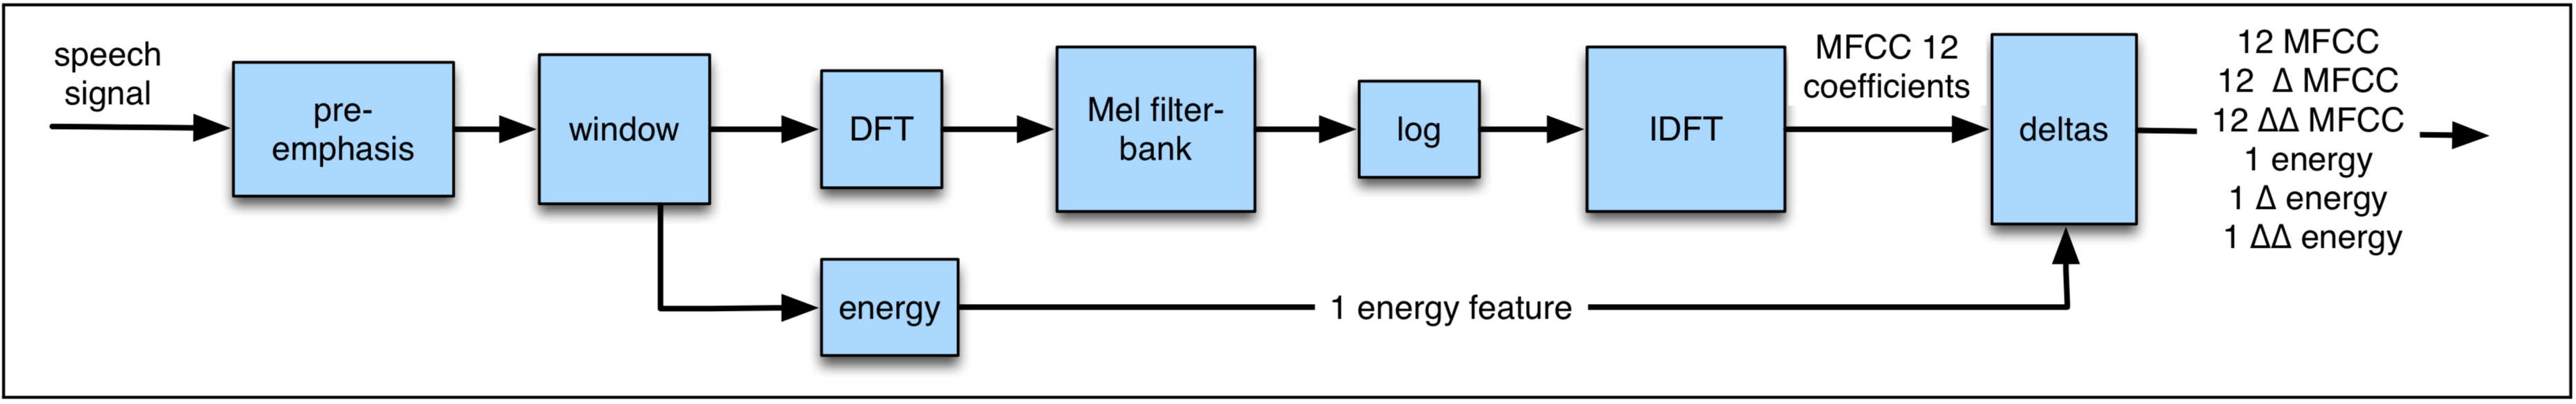
\includegraphics[scale=0.24]{img/mfcc-extraction.png}
\caption{The extraction of sequence 39-dimensional MFCC vectors from a waveform.}
\label{fig:vc-flowchart}
\end{figure}

\subsection{Gaussian mixture models}

A Gaussian mixture model is a type of probablistic model that aims to
represent normally distributed groups within a set. This is based on the
idea of the normal, or \emph{Gaussian} distribution, which can be see in
\autoref{fig:gaussian-dist}.
\colorbox{magenta}{[Create new graph from scratch or cite it.]} The
Gaussian distribution is characterized by two main features: the mean
(the arithmetic average of the data) and the variance (the spread of the
data from the mean). The Gaussian distribution is the most important
distribution used in probablistic modelling as it has been theorized
that the average of independent random variables would look like a
normal distribution \parencite{mcgonagle2016}.

\begin{figure}[ht!]
\centering
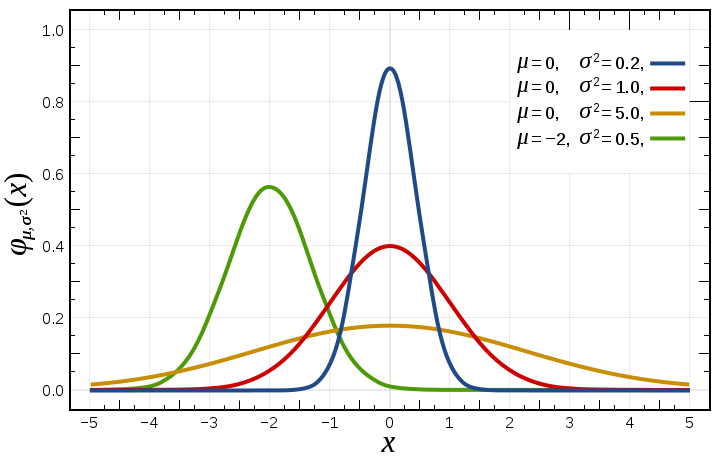
\includegraphics[scale=0.40]{img/gaussian-dist.png}
\caption{The Gaussian distribution with different means (\( \mu \)) and variances (\( \sigma^2 \)).}
\label{fig:gaussian-dist}
\end{figure}

Gaussian mixture models are based on the principle that if a unimodal
(one `peak') dataset can be fit with a Gaussian distribution, then a
multimodal (multi `peak') dataset is just a `mixture' of smaller
Gaussian distributions. A common example given to understand the
Gaussian distribution and Gaussian mixture models often references
height. It is often said that men are taller than women on average, with
men being 178cm (5 foot 10 inches), and women being 165cm (5 foot 5
inches). If we used two separate Gaussians to model each gender, we
could `mix' them to model the likelihood of a certain data point
(e.g.~person) being a male or a female \parencite{mcgonagle2016}. For
example, using a hypothetical example with the averages previously
mentioned, we could see that the likelihood of a person that is 168cm is
more likely to be a male than a female. This is demonstrated in
\autoref{fig:gmm-height}.
\colorbox{magenta}{[Create new graph from scratch or cite it.]}

\begin{figure}[ht!]
\centering
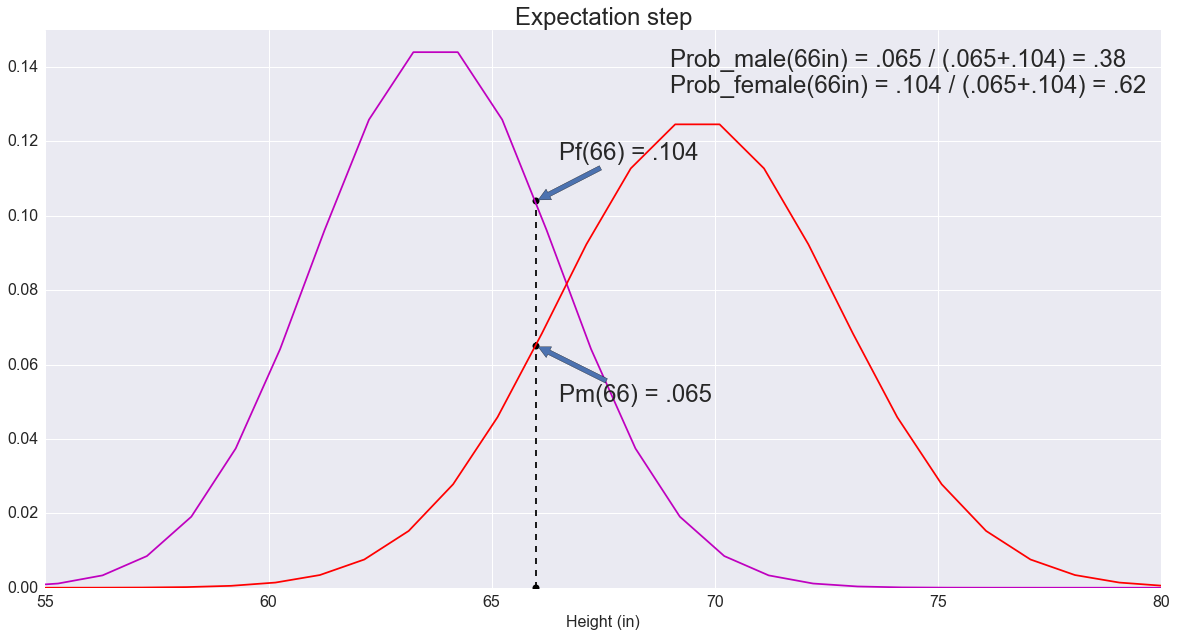
\includegraphics[scale=0.30]{img/gmm-height.png}
\caption{An example of a GMM using male and female height. The likelihoods for each gender for someone 168cm (66in) tall is calculated using the percentage of men and women in the dataset from the vertical axis. The probabilities are given in the top right corner.} 
\label{fig:gmm-height}
\end{figure}

However, as simple as this sounds the most advantageous point of the
Gaussian mixture model is the fact that it is an \emph{unsupervised}
model that can be used when the subpopulations of the data are unknown.
Thus, following the previous example of height, a Gaussian mixture model
could be used to model the height of the two genders \emph{without}
knowing the gender of each datapoint.

Because it is an \emph{unsupervised} model, it requires a special method
to estimate the appropriate parameters. The most common method used for
this is known as \emph{expectation maximization}. This algorithm is used
for maximum likelihood estimation. In other words, this algorithm tries
to find the most appropriate group for each datapoint by calculating the
probability of it being in a certain group and selecting the most likely
one. This is done iteratively by initializing reasonable values, and
then calculating the probability of membership in each cluster (the
\emph{expectation} step) and updating each clusters location,
normalization and shape using the probabilities calculated (the
\emph{maximization} step) until the algorithms converge
\parencite{vanderplas2016}. A visual example of the convergence process
taken from \textcite{mcgonagle2016} can be seen in
\autoref{fig:em-converge}.

\begin{figure}[t!p]
   \centering
   \begin{subfigure}[b]{0.4\textwidth}
      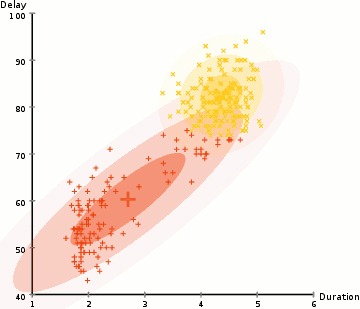
\includegraphics[width=1\textwidth]{img/em-alg2.jpg}
         \caption{Initizalization}
         \label{fig:gmm-init}
   \end{subfigure}
   \quad
   \begin{subfigure}[b]{0.4\textwidth}
      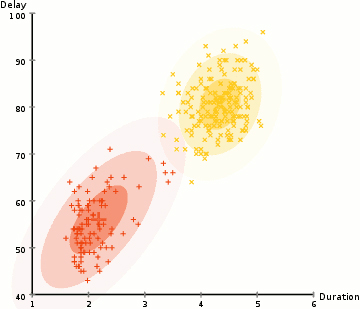
\includegraphics[width=1\textwidth]{img/em-alg3.jpg}
         \caption{Mid-convergence}
         \label{fig:gmm-mid}
   \end{subfigure}
   
   
   \begin{subfigure}[b]{\textwidth}
      \centering
      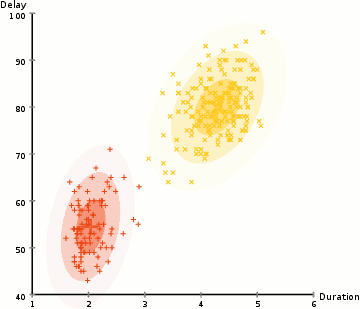
\includegraphics[width=0.45\textwidth]{img/em-alg4.jpg}
         \caption{Converged}
         \label{fig:gmm-conv}
   \end{subfigure}
   \quad
   \caption{Gaussian Mixture Model convergence using the Expectation-Maximization algorithm.}\label{fig:em-converge}
\end{figure}

This model can be compared to the \emph{k}-means clustering algorithm,
as both can be used to cluster different subgroups. Like the
\emph{k}-means algorithm, GMMs also require us to specify a number of
components, which usually indicate the number of subgroups we hope to
cluster. However, \emph{k}-means suffers from not using a probablistic
model to assign clusters, which means that data points can only be
assigned to exactly one cluster. The cluster shape of \emph{k}-means is
also limited to only circles, which makes it inadequate to model data
with different distributions. GMMs manage to address these issues by
using the expectation-maximization algorithm to calculate the
probabilities of cluster assignment and by allowing for different
covariance types which permits for different cluster shapes beyond the
circle. Aside from being useful as an unsupervised classification
algorithm, GMMs can also be seen as a generative algorithm as it models
the overall distribution of the data \parencite{mcgonagle2016}. This
means that a GMM can be used to generate new data points following the
distribution of the given data set.

In the case of speech, Gaussian mixture models are most often used to
model individual sounds using MFCC feature vectors. Because MFCC feature
vectors are multi-dimensional
(\begin{math} \sim \end{math}39-dimensions), the Gaussians within the
model are also multi-variate. However, the same principles described
above still stand, and allow us to calculate the probability of a sound
from a given frame.

Although GMMs are useful for modeling the distribution of sounds within
a dataset and allow us to generate any observation, they are only
capable of modeling speech as discrete MFCC vectors as opposed to a
continuous sequence. Thus, GMMs are often utilized with Hidden Markov
Models to remedy this issue. In short, Hidden Markov Models are models
that consist of \emph{states} and \emph{transitions}. When utilized in
speech recognition, each state represents a potential sound, while the
transitions represents the probability or likelihood of the next state
(e.g.~sound). Gaussian mixture models can be used to represent a sound
within a state
\colorbox{magenta}{[check from here; this also needs a diagram]}.

\subsection{Neural networks}

As indicated by its name, neural networks or more formally,
\emph{artificial neural networks} are said to be based on the
architecture of the brain's neurons. Like the human decision making
process, neural networks take in a certain amount of information or
\emph{input}, to make a decision, or more formally, to give an
\emph{output}. This idea can be easily understood by taking a look at
the \emph{perceptron}, the most simple form of an artificial neuron.

\begin{figure}[ht!]
\centering
\includegraphics[scale=0.20]{img/perceptron.png}
\caption{A visual representation of the perceptron.}
\label{fig:perceptron}
\end{figure}

A perceptron takes in a number of binary inputs (represented in the
image by \begin{math} x_1, x_2, x_3 \end{math} ) and outputs a single
binary output \parencite{nielsen2015}. The output is determined by
whether the inputs are less than or greater than a defined threshold,
and each input can be weighted to represent the importance of that input
in determining the output. Mathematically, this can be represented as
the following:

\begin{equation*}
    output=\begin{cases}
        0 & \text{if $\sum_{j} w_jx_j \leq$ threshold} \\
        1 & \text{if $\sum_{j} w_jx_j >$ threshold}
    \end{cases}
\end{equation*}

To provide a concrete example, we can use a yes-no question (with 0
representing `no', and 1 representing `yes') such as:

\emph{``Will I watch another episode of this TV show?''}

As `inputs', we can use the following questions:

\begin{enumerate}
\def\labelenumi{\arabic{enumi}.}
\tightlist
\item
  Do I like this show?
\item
  Is it still before my bedtime?
\item
  Am I free tomorrow?
\end{enumerate}

To decide the weights of these `inputs', we can consider how important
we think each question is. Perhaps the most important question is
Question \#1, and thus we can assign a weight of 4, while the other 2
may receive a weight of 2 and 1.

Finally, we need to define a threshold to determine whether we output a
0 (no) or a 1 (yes). Evidentally, the lower the threshold, the more
likely we're going to watch another episode. For example, with the given
weights and a threshold of 2, we have the following possible outputs for
each question:

\begin{enumerate}
\def\labelenumi{\arabic{enumi}.}
\tightlist
\item
  4 * 1 = 4 OR 4 * 0 = 0
\item
  2 * 1 = 2 OR 2 * 0 = 0
\item
  1 * 1 = 1 OR 1 * 0 = 0
\end{enumerate}

We can see that we would end up with a final output of 1 (yes) in the
case that it is still before our bedtime (2 points) and/or if we like
this show (6 points/4 points), and regardless of whether we are free
tomorrow.

Even though the previous notation of the perceptron is more simple, the
perceptron, and more generally speaking, the neuron is more often
described in the following notation where w represents a vector of the
weights, x represents a vector of the inputs, and b represents
\emph{bias}, to replace the threshold.

\begin{equation*}
    output=\begin{cases}
        0 & \text{if $w * x + b \leq$ 0} \\
        1 & \text{if $w * x + b >$ 0}
    \end{cases}
\end{equation*}

The bias can be understood as being equivalent to -threshold. It can
also be understood in terms of the neuron metaphor of how easy it is to
get the neuron to `fire'. That is to say, the bigger the bias, the more
likely we output a 1, and the smaller the bias, the more likely we
output a 0.

Although perceptrons are very simple to understand, they tend to not
function well in more complex situations due to their structure. In
particular, a small change in the weights could easily cause the output
to go from a 1 to 0 and vice versa. Of course, in the case of the
example above, this may not matter too heavily, but in training large
systems, this property is too afflicting to be reliable
\parencite{nielsen2015}.

Instead, the most basic neuron used in machine learning is the
\emph{sigmoid} neuron, which as the name indicates, utilizes the sigmoid
function to decide the threshold. This prevents the neuron from being
affected by small changes like the perceptron, as the decision function
is no longer linear. The sigmoid neuron is also much more flexible, as
it no longer requires a binary input and can instead take on any values
between 0 and 1. Aside from the sigmoid, there are other non-linear
functions that can be used, such as the tanh function or another known
as the rectified linear unit (ReLU) which can offer slight improvements
over the sigmoid depending on the task. In general, these non-linear
functions are what give neural networks their vast power to `learn'
\parencite{nielsen2015}.

While a single neuron may be able to make very basic decisions, it is
through a combination of them that we can make more complex systems that
do tasks such as named entity recognition, object detection and voice
conversion. From here, we get the name of neural \emph{network}. In the
following figure, we see an example of a more typical neural network.

\colorbox{magenta}{[Replace image below]}

\begin{figure}[H]
\centering
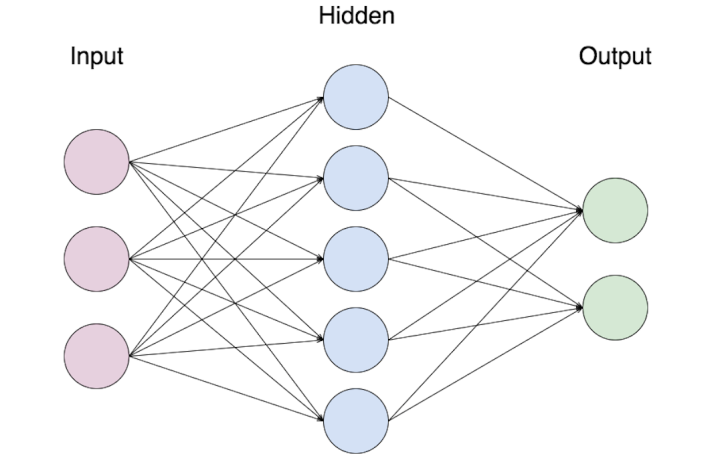
\includegraphics[scale=0.35]{img/neural-network.png}
\caption{An example of a neural network.}
\label{fig:neural-network}
\end{figure}

In the example above, we have three inputs and two outputs, and a new
concept known as a \emph{hidden layer}. The hidden layer is said to be
able to `uncover' more additional information about the input in order
to better decide the output. While the current example only has one
hidden layer, the currently popular `deep learning' comes from adding
multiple hidden layers to create a large neural network structure. Like
hidden layers, the number of inputs and the number of puts can vastly
vary depending on the dataset. For example, in the case of
part-of-speech tagging, we would like the input and output size to be
the same per sentence, as we need to have a part-of-speech tag applied
to each word. The output layer can the output the probability of each
possible part-of-speech tag (noun, verb, adjective, etc.) per word, and
we can select the most probable as that word's part-of-speech.

While neural networks are described at a high level here in order to
facilitate general understanding of this work, more complex neural
network architectures and features are not addressed here. Further
reference regarding neural networks can be found in
\textcite{nielsen2015}, the main reference for the description here, and
\textcite{goldberg2017}, which provides both an overview on neural
networks and discussion of their use in natural language processing.

Neural networks in the context of voice/accent conversion will be
further described in \autoref{accent-conversion} and
\autoref{experiment-2-i-vector-based-accent-conversion}.
\chapter{Literature Review}

This section provides a brief overview of second language acquisition
and education in order to frame the challenge of pronunciation and to
motivate the potential usage of technology in language learning. I then
examine some previous research in spoken language technology used in the
domain of language education, including discussion on computer assisted
pronunciation (CAPT) systems in order to shed light on where voice
conversion and accent conversion could be applied, and then detail some
important pivotal work done in the two areas.

\hypertarget{theoretical-and-educational-motivations}{%
\section{Theoretical and educational
motivations}\label{theoretical-and-educational-motivations}}

Linguists have long debated over the possibility of whether second
language (L2) learners (e.g.~adult learners) could ever acquire a
language to the extent of a native speaker. Some still cite ideas like
the Critical Period (CP) Hypothesis and neuroplasticity which claims
that learners cannot acquire language (at least as well as a native
speaker) after a certain point in time due to the loss of plasticity in
the brain \parencite{lenneberg1967a,scovel1988a}. This theory has been
particularly cited in reference to pronunciation, perhaps due to the
obvious difficultly in overcoming the L1 negative transfer (e.g.~effect
of our native language) that many, if not all, language learners
experience in speaking a new language.

Since the emergence of the CP hypothesis, many linguists have
investigated the relationship between a number of variables such as age,
motivation, and language use, that interact with the level of language
acquisition. \textcite{piske2001} and \textcite{lengeris2012} present an
excellent review of different literature that investigates the
interactions between these various variables and their effects on
foreign accent. They discuss that although many L2 foreign accent
studies do support the idea that the earlier a language learner learns a
language, the better their accent would be, there isn't strong enough
indication to support the notion of a `critical' period. They do concede
that many studies do indicate that there is a linear correlation between
age and foreign accent, but this only indicates a `sensitive' period,
not a `critical' period, a distinction that some fail to acknowledge.
That is to say, following advocates of the CP, the critical period
should end roughly around 12 years old \parencite{scovel1988a}, or no
later than 15 years old \parencite{patkowski1990}, and beyond this
point, there would be ``a sharp drop-off in a learner's abilities''
\parencite{lengeris2012}, indicating that a learner could not acquire a
native-like accent beyond this period.

Other researchers such as \textcite{long1990} suggested that an L2
learner could speak accent-free if they learned the language before 6
years old but not after 12 years old. Although this notion also has been
supported through a number of studies, there has also been
counter-evidence found in other studies that found that there were
learners younger than 6 who had detectable traces of a foreign accent.
In other studies that examined learners of English who started beyond 12
years old, they also found evidence of learners with no detectable
foreign accent. For example, in \textcite{flege1995}, it was found that
6\% of 120 native speakers of Italian who started learning English after
the age of 12 years old had native-like pronunciation, and in
\textcite{bongaerts1995}, it was found that 5 out of 11 speakers were
rated comparable to the native English control subjects. Thus
\textcite{piske2001} conclude that while there is evidence that earlier
learners can learn an L2 with less chance or degree of a foreign accent,
this does not necessarily support the CP hypothesis or the idea that the
loss of plasticity in the brain leads to an inability to acquire
language.

Following their review of the correlation between other potential
variables and the degree of foreign accent, \textcite{piske2001} take a
further look at \textcite{bongaerts1995}. Although it was found that 5
out of 11 speakers were perceived as \textit{indistinguishable} from
native English speakers, \textcite{piske2001} also point to a number of
other factors in play that could have potentially allowed these speakers
to be perceived as such. Perhaps the most controversial factor is the
fact that these speakers were native Dutch speakers. Because Dutch and
English have a similar phonetic inventory, it has been argued that this
allows for easier acquisition of a native-like accent. In examination of
their motivation, these learners were considered highly motivated as
they felt the need to speak English without a Dutch accent due to their
positions as university-level English teachers. On top of this, these
learners also received intensive training in the perception and
production of English sounds. Examining the interaction between these
variables, it may be appropriate to conclude that the reason why 5 out
of the 11 speakers were evaluated as indistinguishable from native
speakers is due to the fact that they are a very niche population.

Regardless, this points to the fact that there is the possibility of
language learners acquiring native-like pronunciation given the right
configuration, even if the said configuration may be difficult to
achieve. This is contrary to what is suggested by the CP hypothesis,
which suggests that \emph{all} learners are limited by a critical
period. This is not to say that learners are not still deterred by a
`sensitive period', but this does highlight the potential that learners
could be taught pronunciation should they have the right tools.

Aside from the issue of whether or not language learners could ever
achieve native-like performance, another question that arises is whether
or not there is even a \textit{need} for learners to aim so high. In
\textcite{munro1999}, they discuss the interaction between foreign
accent, comprehensibility and intelligibility and point out that the
goal for many L2 learners is to communicate and not necessarily sound
like a native speaker. Thus while there are unique groups of learners
like those from \textcite{bongaerts1995}, \textcite{munro1999} point out
that most learners strive for effective communication. In order to
observe the interaction between foreign accent, comprehensibility and
intelligibility, a they conduct a perceptual study on the performance of
native Mandarin speakers. Following this study, they found that despite
the fact that some speakers may have what some consider a `heavy
accent', this does not automatically mean that they are unintelligible.
However, they do cite that some accents may cause longer processing
times than others. When observing the interaction of variables such as
phonemic errors and intonation with intelligibility and
comprehensibility, they found that intonation was the most influential
factor in comprehensibility, while phonemic errors affected
intelligibility. This substantiates the concepts of comprehensibility
and intelligibility themselves, as intelligibility is the degree a
speaker is understood without involving interpretation (e.g. ``What did
they say?''), while comprehensibility is the degree a speaker is
understood in terms of meaning (e.g. ``What do they mean?''). Thus, they
suggest that successful communication requires attention to both sounds
and prosody for better comprehensibility and intelligibility.

While linguists make these discoveries and observations of L2 learning,
it seems that it takes a lot of effort for them to trickle down to the
foreign language classroom. In \textcite{darcy2012}, they find through a
small survey of 14 teachers that although teachers tend to find
pronunciation to be `very important', the majority do not teach it at
all. When asked why they do not teach it, they cited reasons such as
`time, a lack of training and the need for more guidance and
institutional support'. Even though the number of teachers surveyed may
be significantly small, this gives us a glimpse through the lens of what
language teachers themselves experience in relation to pronunciation. We
see that even though teachers would like to address it, this would
require a restructuring in their curriculum and training-- something
that would undoubtedly take even more time before students get more
pronunciation attention. Compounded with the issue of time and the fact
that not all learners need or want equal amount of pronunciation
training, it may be unlikely to see such change in second language
curriculum so soon.

This points to the potential solution of employing a technology-based
system to improve pronunciation as learners could individually address
their needs \textit{outside} of the classroom.

\hypertarget{spoken-language-technology-for-education}{%
\section{Spoken language technology for
education}\label{spoken-language-technology-for-education}}

Over the decades, as speech technology has slowly evolved and started to
show its potential, many researchers have tried to test its limits by
innovating a number of systems to address the challenge of
pronunciation. Included in these systems are systems such as
computer-assisted pronunciation training (CAPT) systems which attempt to
tutor pronunciation through explicit teaching as well as more modern
gamified techniques, which attempt to coerce language learners in to
practicing pronunciation by making the process more engaging.

Among the two, CAPT systems have had more history due to the extra
development and testing gamified techniques require. In fact, gamified
systems can be considered a subclass of CAPT systems, as both require a
fundamental setup in order to assist the language learner. In general,
these systems utilize some form of automatic speech recognition (ASR) to
record a speaker and compares their recordings (usually) with a native
speaker gold standard. They also usually include a feedback mechanism
with a combination of pitch contours, spectrograms or audio recordings
to help the user adjust their pronunciation, with gamified systems
including at least a point mechanism to motivate the user.

In order to understand the connection between language education and
spoken language technology, we take a look at \textcite{neri2002} where
we a presented with a through overview between the two areas. Here, we
see that aside from the classroom, there seems to be an issue in
relating the findings of linguistics/language pedagogy with technology.
Part of the reason, they suggest, stems from the fact that there are not
`clear guidelines' on how to adapt second language acquisition research
and thus many CAPT systems `fail to meet sound pedagogical
requirements'. They emphasize the need for the learners to have
appropriate input, output, and feedback and exhibit how the systems
available at the time were lacking. For example, they criticize some
CAPT systems that were prevalent at the time including systems like
\textit{Pro-nunciation} and the \textit{Tell Me More} series for
utilizing feedback systems that give the users feedback in waveforms and
spectrograms, which cannot be easily interpreted without training.
Further, they argue that although visual feedback has its merits, this
kind of feedback suggests to the user that their utterance must look
close to what is shown on the screen, which is not the case. An
utterance can be pronounced perfectly fine, but look completely
different from a spectrogram, and \textit{especially} a waveform due to
the number of features represented in each visualization, such as the
intensity, which will indefinitely vary from user to user and the given
examplar. They conclude their article by making it a point to discuss
recommendations for CAPT systems, by stating that they should integrate
what has been found in research from second language acquisition, and to
train pronunciation in a communicative manner to give context to the
learners. They also point to the problematic area of feedback and advise
that systems provide more easily interpretable feedback with both audio
and visual information, and propose that systems give exercises that are
`realistic, varied, and engaging'. Although this article was first
published in 2002, it outlines a good fundamental structure that CAPT
systems require-- something that many systems still seem to be lacking.

In \textcite{eskenazi2009}, we are given a more technical review of CAPT
systems with attention to the different CAPT system types and their
limitations as well as some discussion on prosody detection.

The article explains that CAPT systems can be generally split into two
main types: individual error detection and pronunciation assessment. As
indicated, individual error detection systems are more focused on one
particular aspect of the user's speech, such as the phones or pitch,
while pronunciation assessment systems are more designed to represent
how a human would judge a non-native utterance.

Early individual error detection systems, including one of the author's
very own \textcite{eskenazi1998}, started by using a variety of speech
recognition techniques such as forced alignment or unconstrained speech
recognition. They also worked with a variety of measures to detect the
differences between the individual errors and gold standard. Some of
these measures include hidden Markov model (HMM) based recognition
scoring, a confidence score based system known as Goodness of
Pronunciation (GOP), and Linear Discriminant Analysis (LDA). Each of
these measures were found to somehow detect the users' errors; however
they suffer from issues like low precision or the need for a very
homogeneous sample (e.g.~Japanese speakers).

Although some of these early systems showed some signs of promise, they
tended to over-simplify the issue of pronunciation training.
\textcite{eskenazi2009} makes a point of this by emphasizing the fact
that improving non-native pronunciation is not simply a binary question
of native vs.~non-native. Instead the L1 of the system's users must be
considered as this in itself can greatly affect the evaluation.
\textcite{eskenazi2009} also points out that the level of language
learning of the speakers can also impact the metrics and success of the
system as well, and thus an appropriate population must be selected
carefully when building a CAPT system, especially when considering
individual errors.

In examining previous CAPT systems, \textcite{eskenazi2009} briefly
discusses prosody correction, an often overlooked area as previously
mentioned. \textcite{eskenazi2009} points to some pivotal works that
have used a variety of methods to address the issue, including systems
that use Pitch Synchronous Overlap and Add (PSOLA) to resynthesize the
prosody of users to help them hear what an appropriate utterance would
sound like. This has been suggested to be a potentially effective
feedback mechanism to employ in future systems, as it has been said that
imitating one's own voice is the most effective \parencite{felps2009}.
Among prosody correction systems, \textcite{eskenazi2009} mentions two
main types-- those that use appropriate L2 phonological models and break
prosody down into two levels--- syllable-word and utterance-phrase, and
systems that detect the `liveliness' of a speaker. However, these
systems require tuning of a variety features including F0, power,
duration or phonetic transcription, which makes it difficult to
automatically create the necessary adjustments not just
cross-linguistically, but across speakers as well.
\textcite{eskenazi2009} concludes by stating that although such
limitations exist in these systems, the usage of ASR and other speech
technologies has grown from such a sparse beginning, and that because
the market appeal for such systems is large, they shall soon serve
central roles in language education.

Aside from general discussion on CAPT systems, \textcite{chun2008}
present a review of other technologies used in pronunciation training,
with emphasis on feedback mechanisms used to train prosody. They discuss
four main tools used in teaching prosody: `visualization of pitch
contours', `multimodal tools', `spectrographic displays' and `vowel
analysis programs'. Citing previous work, it appears that they suggest
that the visualization of pitch contours is the most robust method of
feedback for learners as it is the most intuitive and non-language
specific. Aside from this however, they also discuss the potential of a
multimedia approach used by \textcite{hardison2005} that integrate both
audio and video in a system called \textit{Anvil}. Following this
research, users of this system were able to generalize their training
beyond a sentence level and were able to perform better at a
discourse-level. This methodology encapsulates a good feedback mechanism
as described by \textcite{neri2002} as it provides adequate feedback by
being easily interpretable, stimulates both audio and visual channels
and puts the language in context.

\textcite{chun2008} also discuss the two main methods of such prosody
systems: one which utilizes isolated scripted sentences and the other
utilizing imitation. While both types of systems are common, possibly
due to their easier implementation, they conclude that neither method is
useful for generalizing to novel speech production. Aside from the fact
that the language may not be put into context, one problem with both
types of systems is their limited number of sentences and limited source
speakers in terms of imitation. This prevents learners from gaining an
understanding of the variability of acceptable (and hence unacceptable)
prosody across speakers and contexts, and may limit learners to speaking
as similarly as they can to the given exemplars. Thus, while these
systems might provide language learners with a basis to improve their
prosody, further work needs to be put in to help them contextualize
prosody as a general concept and to give learners more autonomy in
developing their own speaking style.

Similar to \textcite{neri2002}, \textcite{chun2008} also gives insight
on potential ways to improve future CAPT systems. One particularly
compelling suggestion they give is to expand systems to include gestures
and movement. While most research on language education and in turn,
linguistics, is focused on the spoken aspect, \textcite{chun2008} points
out that spoken language is complementary with our body language. For
example, when we raise our pitch, we also tend to raise our eyebrows and
chin, and when we emphasize a specific, we might also stress it by
opening our eyes slightly wider, bobbing our head or pointing our
finger. In fact, one of the few studies that examine the effect of
including body language in teaching L2 listening comprehension found
that learners performed much better with these visual cues as opposed to
only having audio cues. Thus they conclude that in order to create
better pronunciation training systems, learners must be provided with
better feedback and language must be placed into context not only in
terms of real-life situations, but also in terms of communication as a
whole by including gestures and movement.

With that said, building pronunciation systems that take all of the
previous suggestions into consideration requires adept planning and
expertise, and can be demanding for most research groups. Instead, some
of have tried to adapt already existing technology and build a small
architecture around it. For example, \parencite{tejedor-garcia2017}
experiment with utilizing synthetic voices for corrective feedback in a
pronunciation training tool. In their study, they use Google's offline
Android text-to-speech (TTS) system as feedback for B1 and B2 Spanish
learners of English, and have them focus on the six most difficult pairs
of vowels \colorbox{magenta}{[insert IPA here?]}. In order to train the
users, the researchers first had them watch videos that describe the
articulatory/perceptive features of the vowels, and had them listen to a
number of minimal pairs produced by the TTS system in succession.
Afterwards, they were asked to discriminate minimal pairs in a listening
task and then asked to pronounce them. From this study, they conclude
that making use of commercial TTS systems are beneficial for users and
instructors alike as indicated by both the improvement in performance by
the users and the feedback given by those involved in the experiment.
However, because the study was limited to individual words and only six
pairs of vowels, further experimentation needs to be conducted in order
to understand whether these learners can generalize their training.

Through examining these various works, it is evident that there is a
large potential for appropriately adapting technology to guide and help
language learners and teachers alike. Yet, in order to provide
long-standing worthwhile results, further consideration needs to be
given to the suggestions and evidence of previous research and should be
integrated in the design and implementation of future systems. This
implies that the appropriate time and resources may need to be dedicated
in order to push the boundaries of CAPT systems.

\hypertarget{voice-conversion}{%
\section{Voice conversion}\label{voice-conversion}}

There have been a number of efforts to design voice conversion systems
using various methodologies. Much like the rest of the speech technology
field, earlier voice conversion systems began with utilizing MFCCs and
GMMs for conversion and slowly evolved towards utilizing more advanced
features and adaptation techniques.

In particular, a variation of GMM voice conversion set forth by
\textcite{toda2007} has become what appears to be the standard set-up.
Following their reasoning, they argue that although regular GMMs perform
fairly well in voice conversion, they also lead to the deterioration of
speech quality. Instead, they propose that by using a maximum-likelihood
estimation of the spectral parameter trajectories, issues that cause the
loss of quality such as oversmoothing of the spectral features can be
avoided. They provide detailed theoretical evidence to support their
method which can be further observed by taking a look at their paper.

GMMs have long been used for voice conversion alongside other speech
tasks, but more recently another method-- or more accurately another
feature in place of MFCCs, known as \emph{i-vectors} have taken off. To
put concisely, i-vectors are akin to word embeddings in text-based
natural language processing tasks in the sense that i-vectors
encapsulate any type of desired speech information in a vectorized
fashion. This may be confusable with MFCCs, which also vectorize speech
information; however MFCCs specifically vectorize individual speech
sounds from frames, while i-vectors tend to vectorize more large-scale,
dynamic speech information.

The usage of i-vectors have proven to be successful in a number of
tasks, such as speaker verification, language identification, and native
accent identification. They have become especially popular due to the
fact that they work well with unlabeled acoustic data. Referring back to
the overview of voice conversion in the previous section, it is
mentioned that labeled acoustic data often leads to better results in
the conversion, but is also often unavailable. Thus i-vectors are able
to fill this gap in the lack of available labeled data and the loss of
conversion quality.

In the instance of voice conversion, i-vectors are made of speaker
super-vectors trained on GMMs and low dimensional features that
represent an individual speaker's features \parencite{wu2016}. This is
extracted per utterance and then averaged to form an i-vector that
represents an individual speaker. In this way, a source speaker's
i-vector can be approximated towards a target speaker's i-vector by a
mapping function using neural networks, gaussian mixture models, or
other appropriate algorithms.

The usage of i-vectors in voice conversion has been seen in works such
as \textcite{wu2016} and \textcite{kinnunen2017}. Following
\textcite{kinnunen2017}, the usage of i-vectors in voice conversion
aligns perfectly with the task as it is highly similar to speaker
verification; however instead of being a classification task (e.g.~is
this said speaker or not), voice conversion is a regression task. In
\textcite{wu2016}, they test and compare the performance of using plain
mel-cepstral coefficients (MCCs) against i-vectors by training a variety
of systems. Among their systems, they utilize a strategy known as the
\emph{average voice model}, which models what an average speaker would
sound like by utilizing a large amount of parallel utterances, which
also allows for conversion between two speakers \emph{without} having
parallel utterances. In order to compare MCCs vs.~i-vectors, they train
systems using MCCs as features with a deep bi-directional long-short
term memory neural (DBLSTM) network architecture, a DBLSTM combined with
an average voice model (DBLSTM + AVM), and a DBLSTM combined with an
average voice model retrained on some paralleled data from the testing
source-target speakers (DBLSTM + RM). They then train another system
with i-vectors using the DBLSTM and average voice model (DBLSTM + AVM +
i-vectors). In order to evaluate these models, they provide both an
objective evaluation using a measure known as mel-cepstral distortion
(MCD) and a subjective evaluation rated on quality and similarity, which
was decided by the votes of 20 listeners.

Following the results of the objective evaluation, they find that the
system with the lowest mel-cepstral distortion (e.g.~the best system) is
the DBLSTM + RM model, followed by the DBLSTM + AVM model, with the
regular DBLSTM system and DBLSTM + AVM + i-vector system performing
roughly the same. They note that the DBLSTM + RM system likely performed
the best because of the inclusion of parallel data from the test
dataset, while the DBLSTM + AVM outperformed the regular DBLSTM likely
due to the size of the training data. However, they do not give much
indication as to why the DBLSTM + AVM and DBLSTM + AVM + i-vectors
perform similarly. Based off of the MCD alone, it would seem that
i-vectors do not provide much benefit; however they emphasize that the
DBLSTM + RM system does include parallel data while the DBLSTM + AVM +
i-vectors system does not.

In the subjective evaluation, they compare the four systems by using an
ABX preference test to compare: DBLSTM + RM vs.~DBLSTM, DBLSTM + AVM +
i-vectors vs.~DBLSTM + RM and DBLSTM + AVM + i-vectors vs.~DBLSTM + AVM.
With each pair, they have the listeners evaluate 10 sentences for a
total of 200 votes for each system. Following the results, they find
that the DBLSTM + AVM + i-vectors system outperforms the DBLSTM + AVM
system in both the speech quality and speaker similarity categories with
statistical significance, which shows that the average voice model
\emph{without} i-vectors (e.g.~MCCs only cannot capture speaker specific
information. They also find that the DBLSTM + RM system outperforms the
plain DBLSTM system with statistical significance, indicating that the
average voice model is not only useful, but also helps reduce the amount
of parallel training data required to improve the performance. Finally,
they find that the DBLSTM + AVM + i-vectors system was rated slightly
higher in quality, but opposite in similarity. However this was without
statistical significance, indicating that they perform roughly the same.
From this study, \textcite{wu2016} concludes that the DBLSTM + AVM +
i-vectors method has potential as it allows for great flexibility to
generate the target speaker spectrum without using parallel data.

As oppose to \textcite{wu2016} which utilizes the average voice model in
order to create a strong voice conversion system,
\textcite{kinnunen2017} takes a different approach by
\colorbox{magenta}{[hmmm...]}

\textcite{demarco2013}, present a through analysis of the usage of
i-vectors in classifying native British accents.
\colorbox{magenta}{[continue here or move to accent conversion?]}

Even though systematic objective and subjective evaluation against older
methods do indicate that recent methods have improved upon the older
ones, comparing the performance of these systems against a true human
voice, or perhaps more fairly, against other recent systems in other
areas of speech technology, these systems still seem to leave a lot left
to be desired. For example, in listening to the audio of
\textcite{wu2016}\footnote{Visit http://www.nwpu-aslp.org/vc/apsipa-jiewu-demo.pptx to hear samples.}
\colorbox{magenta}{[Maybe change footnotes to say listen to audio on the accompanying disk?]}
it is apparent that regardless of the low quality of the original source
and target audios, the quality of the converted audio sounds muffled.
This can be attributed to the various nuanced steps and features
required to have high quality voice conversion.

For example, in a shared task dedicated to voice conversion,
appropriately called \emph{The Voice Conversion Challenge} where many
leading research groups involved in speech technology around the world
have submitted systems in attempts to tackle the issue. In the second
iteration of the challenge \textcite{lorenzo-trueba2018}, the organizers
proposed both a parallel and non-parallel version of the task, both of
which were evaluated on natural and similarity using crowdsourcing.

The type of systems submitted to the 2018 edition of the task displays
the current state of voice conversion and perhaps machine learning
research in general as this year saw a huge increase in the number of
systems using neural networks. However, it does not go without saying
that there were indeed systems that used more traditional statistical
methods, such as Gaussian Mixture Models (GMM) and one of its
variations, differential GMM (DIFFGMM).

In order to evaluate the systems, a group of roughly 300 listeners were
gathered to carry out a perceptual evaluation. The systems were
evaluated on two main measures: naturalness, which was evaluated on a
scale of 1 (completely unnatural) to 5 (completely natural); and
similarity, which was evaluated using a same/different paradigm.
Following the results, only one system, referred to as N10, was able to
outperform the baseline in terms of naturalness (alongside the original
source and target audios). When observing the performance of other
systems in terms of similarity, we see about 5 our of 23 submitted
systems outperforming the baseline. From this, we can conclude that it
easier to create a system with high similarity than high naturalness,
which is consistent with other common systems.

In discussing the results of the N10 system, the authors credit the
success of the system to the \emph{hundreds of hours} of external speech
data that was utilized to train a model to recognize content-related
features, as well manual fine-tuning. The creators of this system also
made use of WaveNet, a novel high-fidelity vocoder and dozens of hours
of clean English speech, which could also explain the success of their
results. Thus, as previously discussed, we can conclude that creating a
high-fidelity voice conversion requires not only appropriate fine-tuning
of the data, but also a large amount of external data to support the
system.

Thus, even though many systems were neural network based, only one
neural network based system was able to outperform the sprocket
GMM-based baseline, which could suggest that NN-based methods require
proper fine-tuning of the hyperparameters.

Although we see limitations in the systems presented in The 2018 Voice
Conversion Challenge, there have bene other efforts to present high
quality voice conversion systems in works such as and
\textcite{nguyen2016} and \textcite{fang2018}.

\textcite{fang2018} leverages a cycle-consistent adversarial network
(CycleGAN) architecture, a variation of the recently trending generative
adversarial network (GAN) architecture, which was originally used for
unpaired image-to-image translation. For example, GANs have been shown
to be able to convert images of zebras into horses, as well as winter
into summer.

While not necessarily directly related to the standard idea of voice
conversion, there have also been some incredible breakthroughs in
systems set forth by research teams at Google Brain. One such system
involves the Tacotron end-to-end system, which has been proposed to
replace the current set-up of text-to-speech systems by reducing the
amount of components (decoder, vocoder, etc.) into one piece. The
researchers working on this system have recently revealed a impressive
system that also takes advantage of deep neural networks to encode
speaker characteristics into embeddings, which are then utilized to
transfer style \parencite{wang2018}. They show how their system is
capable of transferring a variety of emotions and accents, making the
synthesized audio sound more human-like. Samples of these audios can be
found at the following
link\footnote{Visit \url{https://google.github.io/tacotron/publications/global_style_tokens/} to hear samples.}.

\colorbox{magenta}{Also add to disc?}

Even though the these systems created by Google Brain are highly
impressive, it is evident that the reason for the success of their
systems is due to very fine-grained parameter tuning and the
availability of large-scale, high quality data that many research
institutions likely do not have access to or have funding for. For
example, if we juxtaposed the audio from the Google Brain systems to the
best performing system of the Voice Conversion Challenge 2018, we can
still observe some disfluencies in the audios of the best system of the
VCC 2018. Thus, it may be a long while before the general public has the
ability to completely replicate such systems and before this work
trickles in to the domain of accent conversion.

\hypertarget{accent-conversion}{%
\section{Accent conversion}\label{accent-conversion}}

Due to the specialized nature of accent conversion as compared to voice
conversion, there are fewer articles and systems available for
reference. In fact, most of the recent articles that are easily
accessible on accent conversion were all published by the same group of
researchers at Texas A\&M University.

However, before the work of these researchers, works such as
\textcite{yan2004} and \textcite{huckvale2007}, explored manipulating
various features in order to observe their relationship with a perceived
accent. In \textcite{yan2004}, they manipulate spectral features,
intonation patterns and duration in order to observe their correlation
across British, Australian and American accents. Through an ABX
perceptual test, they found that 75\% of the synthesized utterances were
evaluated as having the native accent, highlighting the potential for
segmental accent conversion.

In \textcite{huckvale2007}, they examine the relationship between
intelligibility and the of morphing various segmental and suprasegmental
features such as pitch, rhythm and segments of an English TTS system
designed to speak `accented' Japanese. This TTS system was designed by
creating a custom dictionary and mapping the Japanese sounds to their
closest English counterpart. They found through native speaker
evaluation that morphing pitch and rhythm individually had no effect,
and similarly modifying segments alone only gave a small improvement.
However, they discovered that combining the morphing of all of these
features created a large increase in intelligibility, with
intelligibility going up from 57\% as seen in their lowest-performing
system to 84\%. The results emphasize the need to consider the
interaction between segmental and suprasegmental in the conversion task.

In one of the earliest works from the Texas A\&M research group, and
perhaps a key influential paper to this work, \textcite{felps2009}
examines the potential of using a method known as Pitch-Synchronous
Overlap and Add (PSOLA) for accent with the motivation of applying it in
the context of language learning. Specifically, they utilize a
specialized PSOLA method known as Fourier-domain PSOLA (FD-PSOLA), as it
performs best in preventing spectral distortion when modifying the
pitch. \colorbox{magenta}{[explain PSOLA]} In order to conduct the
conversion process, they separate the converting of the segments and the
converting of the prosody into two separate parts, with both parts
evaluated individually and combined. In evaluating their method, they
measured the accentedness, acoustic quality and identity of each
converted audio using auditory tests given to a number of speakers.
Similar to \textcite{huckvale2007}, they observe that the combination of
prosodic and segemental transformation lead to a large improvement in
reducing foreign accent. However, in terms of quality, they found that
all transformations led to lower ratings, which likely indicates the
loss of some spectral information. The identity ratings proved to be the
most interesting as \textcite{felps2009} find that the listeners
indicate a `third' speaker. In other words, the converted audio sounds
neither like the source or target speaker. Thus \textcite{felps2009}
concludes that while accentedness is reduced by their system, their
proposed system also loses the necessary information needed to retain
the speaker's identity.

\colorbox{magenta}{\textcite{felps2010}} ? {[}paper on evaluation{]}

\colorbox{magenta}{\textcite{aryal2010}}

\colorbox{magenta}{\textcite{felps2012}}

With that said, \textcite{aryal2014} and other works done by the group
of researchers have made efforts to address the challenge. Throughout
their research, they test a variety of methodologies, including accent
conversion through voice morphing and articulatory synthesis. In the
same work of \textcite{aryal2014}, they propose a variation to standard
forced alignment techniques used in voice conversion to pair frames
based on acoustic similarity.

To achieve this, they first use dynamic time warping (DTW) to align
parallel utterances from the L1 and L2 speakers in order to apply vocal
tract length normalization to dampen the differences in pitch. They then
extract sequences of 24 MFCCs per utterance, and cluster the MFCC
vectors into 512 clusters using the \textit{k}-means algorithm to easily
find the most acoustically similar sound for each frame. The most
acoustically similar frames are then calculated by finding the closest
L2 cluster, and then selecting the most similar frame within the
cluster. After the closest vectors are paired, they map the conversion
using a GMM.

In order to evaluate their system, they had a group of 13 participants
rate 12 utterances from the test set for their perceived accent (Which
utterance was less accented?) and perceived speaker identity (Does
utterance X sound more similar to A or B?). This system was compared to
a standard voice conversion system that uses standard forced alignment
and trained using GMMs. They found that comparing the AC system to the
original L2 audio resulted in participants rating the converted audio as
sounding less accented 86\% of the time, while the VC system compared to
the original L2 audio was rated at 91\% of the time. However, when the
converted audios from both systems were compared, participants rated the
AC system to be less accented compared to the VC system 59\% of the
time. It was also concluded that the AC system was more successful in
retaining speaker identity, as the participants found the converted
audio more similar to the L2 speaker 78\% of the time. More
interestingly, they found that the AC system was especially effective in
converted utterances that are harder for the L2 speaker to pronounce.
This was measured by examining the relationship between the number of
phonemes that do not exist in the L2 language (in this case Spanish),
and the number of listeners who judged the converted speech as sounding
less accented.They found that there was a 0.86 correlation, indicating
the robustness of the AC system. Thus, it appears that adjusting the
alignment method to align acoustically similar sounds is a good start
for accent conversion systems.

\colorbox{magenta}{\textcite{aryal2014a}}

In \textcite{aryal2015}, we see a more novel method that looks beyond
acoustic features to perform accent conversion. Citing the results of
their previous work, they motivate the usage of articulatory gesture
information in accent conversion reasoning that acoustic-based systems
often struggle in the challenge of separating accent from speaker
identity, which causes the accent converted audio to sound like a
combination of the L1 speaker and L2 speaker. To do this, they propose a
system that combines both the more standard acoustic information like
aperiodicity, pitch and energy from the L1 speaker with articulatory
information recording using an electromagnetic articulograph (EMA). Like
many recent works, they test a DNN-based mapping function between the L1
and L2 data, which they compare to the previously popular GMM-based
system.

In the evaluation of their system, they again use crowdsourced efforts
to rate their system based on intelligibility, accentedness, and speaker
identity. According to their sample size of 15 participants, they find
that the DNN-based system was rated to have a 4.3 out of 7 in terms of
intelligibility as compared to 3.84 out of 7 for the GMM-based system,
proving that including articulatory gesture information and DNNs are
more robust in this instance. The participants also rated the DNN-based
system to be more native-like in 67\% of cases as compared to the
GMM-based system. With that said, the test set was only 15 sentences,
which indicates that 10 out of 15 sentences were better with the DNN
system; thus the test set used may be too small to draw hard
conclusions. The most important conclusions drawn from their experiments
was that of the voice identity assessment. In asking the participants to
rate whether an MFCC compression and AC audio from the DNN and GMM-based
systems, they found that the participants were fairly confident that the
two audios were from the same person with both systems, with the
DNN-based system outperforming the GMM-based system as before at a score
of 4.3 out of 7 on average, and the GMM-based system at a score of 4.0.
However, this is difficult to compare to more common acoustic-only
accent conversion systems, as this is not including in their evaluation.
With that said, it may be possible to conclude that this would
outperform acoustic-based systems, as they proposed this system to
tackle flaws in their previous work.

Evidentally, although including articulatory gesture information seems
to improve the performance of accent conversion systems, as discussed in
the closing remarks of their paper, recording articulatory gesture
information can cost a great deal of money and time
\parencite{aryal2015}. Most publically (and privatized) speech corpora
also do not include this type of information, meaning that experimenting
with it in accent conversion at a broader scale is unfeasibile. Thus, it
is ambitious to accept adding articulatory information to accent
conversion systems and further work needs to be done in order to scale
standard audio-based speech corpora.

Departing from utilizing articulatory gesture information,
\textcite{zhao2018a} returns to a more simpler method similar to
\textcite{aryal2014}. However, instead of matching frames based on their
\emph{acoustic} similarity, they test matching frames based on their
\emph{phonetic} similarity. They do this by mapping the frames of each
source and target speaker into something referred to as a \emph{phonetic
posteriorgram}. Following \textcite{hazen2009}, a phonetic posteriorgram
is `a time vs.~class matrix that represents the posterior probability of
each phonetic class for each time frame'. An example of a phonetic
posteriorgram taken from \textcite{hazen2009} can be seen in
\autoref{fig:phonetic-postgram}.

\begin{figure}[H]
\centering
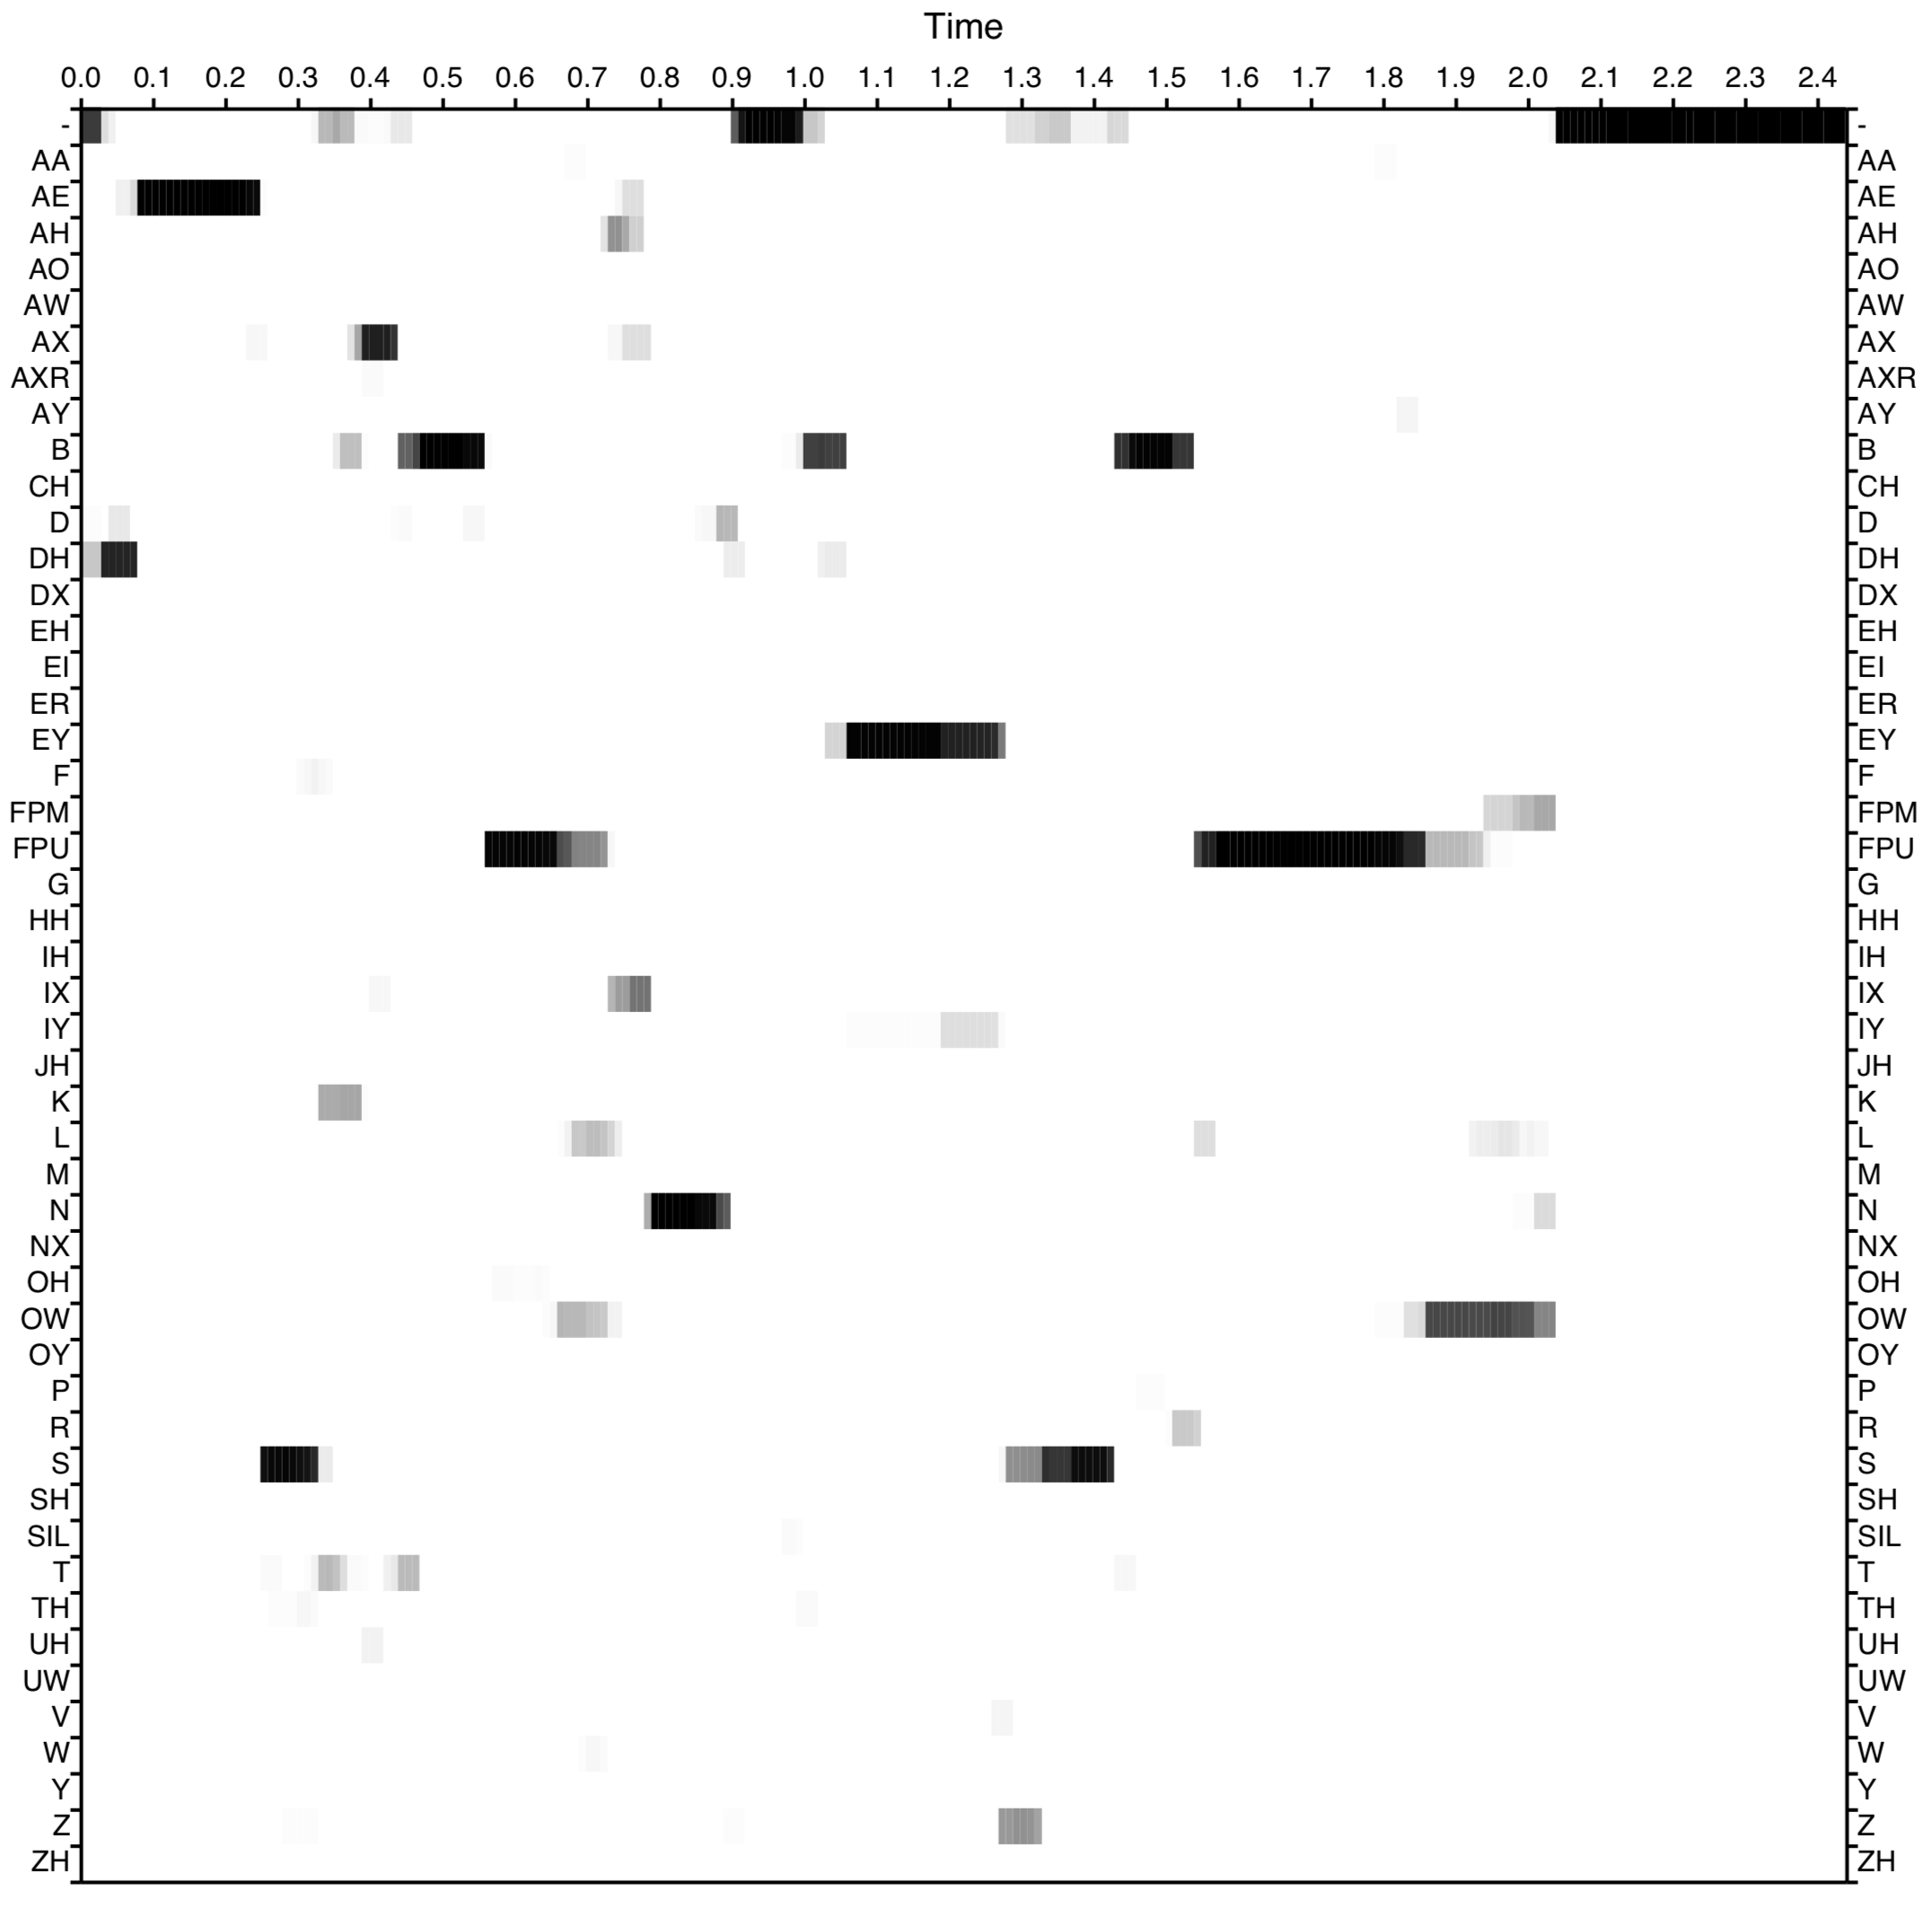
\includegraphics[scale=0.22]{img/phonetic-postgram.png}
\caption{An example posteriorgram representation for the spoken phrase `basketball and baseball'. The x-axis represents the time across the utterance and the y-axis represents the possible phonemes.}
\label{fig:phonetic-postgram}
\end{figure}

The phonetic posteriorgrams are computed using a native English
speaker-independent acoustic model and then the most similar source and
target frames are matched by calculating something known as the
Kullback-Leibler divergence (0 indicating similar or same behavior, 1
indicating completely different) between the source and target
posteriorgrams. After matching the frames, they train GMMs with
128-mixture components to model the distribution of the MCEPs to convert
the speech. The performance of this proposed system is then compared to
a standard voice conversion system using dynamic time warping to align
the frames and the system described in \textcite{aryal2014}.

Like the previous works of \textcite{aryal2014} and
\textcite{aryal2015}, this work also approaches evaluation using a
perceptual listening test to evaluate acoustic quality, speaker identity
and accentedness. However, in this work, they evaluate over 50 test
utterances using 30 participants, which better substantiates their
results compared to the evaluation of 10-15 utterances by 10-15
participants in some of their older studies.

In terms of acoustic quality, they found that their proposed
posteriorgram method received a score of 3.0 on a Mean Opinion Score
scale of 1 to 5 (with 1 being `bad' and 5 being `excellent'), as
compared to a score of 2.6 using the method from \textcite{aryal2014}
and 2.5 for standard voice conversion.

\colorbox{magenta}{[continue]}

Aside from the work conducted by the research group at Texas A\&M
University, it appears to be that there are not many, if any other
researchers currently working in this subarea of accent conversion. This
may be because voice conversion still leaves a lot to be desired itself,
suggesting that most researchers may want to focus on perfecting
standard voice conversion before attempting to tackle something more
fine-grained. However, as research in voice conversion continues to
expand, it also creates the potential to apply methodologies from voice
conversion to accent conversion. Following the general methodologies of
voice conversion, I hypothesize that it should be plausible to convert
accents in a similar fashion and apply more recent innovations to
propose state-of-the-art methods.
\cleardoublepage
\chapter{Design and methodology}

In this chapter, I introduce the dataset and tools utilized in the
experiments, and detail the procedures carried out to conduct the accent
conversion process.

\colorbox{magenta}{Expand this section}

\hypertarget{data}{%
\section{Data}\label{data}}

The main datasets utilized in the following experiments are the Carnegie
Mellon University (CMU) ARCTIC corpus \parencite{kominek2004}, the
L2-ARCTIC corpus \parencite{zhao2018}, a non-native English counterpart
to the CMU Arctic corpus and the Accents of the British Isles (ABI)
corpus. \colorbox{magenta}{cite this!}

\hypertarget{cmu-arctic-corpus}{%
\subsection{CMU ARCTIC corpus}\label{cmu-arctic-corpus}}

The CMU ARCTIC corpus was originally designed to have good phonetic
(specifically diphone) coverage for speech synthesis.
\colorbox{magenta}{Expand this section}

\hypertarget{l2-arctic-corpus}{%
\subsection{L2-ARCTIC corpus}\label{l2-arctic-corpus}}

The L2-ARCTIC corpus currently contains 10 non-native speakers of Hindi,
Korean, Mandarin, Spanish and Arabic, with a male and female speaker for
each language. At the time of writing, the curators of the corpus are
working to add an additional 10 speakers to the corpus by September
2018.

The original audio was sampled at 44.1 kHz, with each recording at
roughly 3.7 seconds on average. In total, the duration of the corpus is
11.2 hours, with each speaker recording an average of 67 minutes of
audio, or the complete ARCTIC sentence prompt list of 1,132 utterances.
However, some speakers did not read all of the sentences and some
recordings were removed as they did not have appropriate quality.

In addition to the audio files, the corpus also includes word and
phoneme-level transcriptions and manually annotated errors for a
150-sentence subset of the corpus, designed to be used in
computer-assisted pronunciation training tools. Within the subset, there
are 100 sentences uttered by all speakers, and 50 sentences that contain
phonemes that are considered to be difficult based on a speaker's L1.
This also includes phone addition, phone substitution, and phone
deletion annotations in ARPAbet format, as well as optional comments
left by the annotators.

\hypertarget{accents-of-the-british-isles-abi-corpus}{%
\subsection{Accents of the British Isles (ABI)
corpus}\label{accents-of-the-british-isles-abi-corpus}}

The ABI corpus was originally designed and collected to support efforts
in systematic studies of the relationship between various accents in the
British Isles and speech technology. At the time of its creation, there
was no appropriate corpus that existed that could be used for this type
of research.

In order to circumvent defining accent, the authors of the corpus
instead chose 14 regions known for their associated accents.

The accents contained in the ABI corpus can be seen in
\autoref{abi-corpus-chart}:

\begin{table}[H]
\centering
\begin{tabular}{|l|l|l|}
\hline
\textbf{Region} & \textbf{Towns/Cities} & \textbf{Code} \\ \hline
Standard Southern English & n/a & sse \\ \hline
Midlands & Birmingham & brm \\ \hline
Wales & Denbeigh & nwa \\ \hline
Scottish Highlands & Elgin & shl \\ \hline
Republic of Ireland & Dublin & roi \\ \hline
East Yorkshire & Hull & eyk \\ \hline
Lancashire & Burnley & lan \\ \hline
Ulster & Belfast & uls \\ \hline
NE England & Newcastle & ncl \\ \hline
Scotland & Glasgow & gla \\ \hline
Inner London & n/a & ilo \\ \hline
NW England & Liverpool & lvp \\ \hline
East Anglia & Lowestoft & ean \\ \hline
West Country & Truro & crn \\ \hline
\end{tabular}
\caption{The regions of the British Isles and their corresponding cities where the ABI corpus was recorded, as well as their corresponding codes in the corpus.}
\label{abi-corpus-chart}
\end{table}

\hypertarget{experimental-data-set-up}{%
\subsection{Experimental data set-up}\label{experimental-data-set-up}}

Using the corpora described above, I split them into two sets of
experiments, with the ARCTIC corpora used in one set of experiments and
the ABI corpus used in another set of experiments.

Following \textcite{zhao2018a} who also works with the ARCTIC corpora,
only 150 utterances or roughly
\colorbox{magenta}{[9 minutes of data] following the L2-ARCTIC average}
are utilized, with the utterances from the L2-ARCTIC corpus downsampled
to 16 kHz to match the quality of the CMU ARCTIC corpus. During the
selection of the 150 utterances, any phrases not recorded by \emph{all}
of the speakers chosen for the experiments were not considered in order
to maintain the parallelness of the experiments.

Although the sample size is very small compared to the actual size of
the corpora, a small sample is chosen to acknowledge the fact that often
only a little amount of data is available or acquirable in building
these systems. This is done similarly in the Voice Conversion Challenge
2018 as well \cite{lorenzo-trueba2018}. The 150 utterances that are used
are chosen at random, but are ensured to be 150 utterances that all
speakers have recorded. Out of these 150 utterances, 100 are randomly
chosen as training utterances while the other 50 are used test
utterances.

\hypertarget{experiments}{%
\section{Experiments}\label{experiments}}

\hypertarget{cmu-arctic-corpus-1}{%
\subsection{CMU ARCTIC Corpus}\label{cmu-arctic-corpus-1}}

As discussed in the introduction of this work, accent conversion has
been proposed as better-suited feedback mechanism for accent training
systems.

The speakers utilized in the experiments are also limited to speakers
BDL (male) and CLB (female) from the CMU ARCTIC database, who are the
native reference speakers, while the non-native speakers chosen from the
L2-ARCTIC corpus are the native Korean speakers (HKK, male; YDCK,
female), Hindi speakers (RRBI, male; TNI, female), and Spanish speakers
(EBVS, male; NJS, female). This is mostly similar to the datasets in
\textcite{zhao2018a}, with the exception of the Korean female speaker
(YDCK) in place of the male Korean speaker (YKWK), which is not included
in the current release (at the time of writing) of the L2-ARCTIC corpus,
and the replacement of the native male Arabic speaker (ABA) with the two
native Spanish speakers.

\hypertarget{abi-corpus}{%
\subsection{ABI Corpus}\label{abi-corpus}}

Accent conversion systems have also been mentioned as a possible
solution to challenges that current speech recognition systems may have.
However, the few accent conversion studies conducted by those from the
Texas A\&M research group have focused on accent conversion between
non-native and native speakers, and voice conversion studies such as the
Voice Conversion Challenge 2016 and 2018 have investigated conversions
between US speakers. Thus, in order to see the effects of accent
conversion between native speakers and to include other varieties of
English, the ABI corpus was chosen.

Although the ABI Corpus contains a total of (HOW MANY?) accents, the
accents used in the experiments were chosen following the DeMarco study.
After organizing the accents into comprehension order, these 3 accents
were respectively the 100\%, 50\% and 25\% different accents.

The ABI Corpus had more coverage in terms of the number of speakers
available per accent and gender, as well as variation in the recording
environment and quality. Concretely, some speakers were much more
quieter than others, while others spoke at a much more rapid pace than
others, or enunciated much less than others. Thus, during the speaker
selection process, I manually listened to a sample of each speaker,
either from the shortphrases or shortsentences folder, and chose based
on these criteria. Some of the chosen speakers had recorded some of the
same words and/or phrases, mostly due to production errors such as
stumbling or reading the wrong word. In the case that a chosen speaker
had repeated recordings, I removed the malformed recordings in order to
keep the experimental corpus as parallel as possible.

The experiments for the ABI corpus are set up similarly to the ARCTIC
experiments in terms of the proportion of training and test set
utterances. However, unlike the ARCTIC corpus, the total amount of data
available for the ABI corpus was less (INSERT TIME IN MINUTES).

Because the ABI corpus contains a large number of accents and speakers,
I chose one accent as the source accent for all conversions, and three
separate accents as the target accents. Specifically, I chose the
Standard Southern English accent as the source accent as it

\hypertarget{tools-and-set-up}{%
\subsection{Tools and set-up}\label{tools-and-set-up}}

In order to understand more traditional mapping methods used in voice
and accent conversion, I follow the methods described in
\colorbox{magenta}{[something about Toda (2007)]} for voice conversion
and reimplement the method described in \textcite{aryal2014} which
utilized frame matching based on acoustic similarity.

In reimplementing \textcite{aryal2014}, certain features were removed--
namely vocal length tract normalization and prosody modification.
Although it is discussed that vocal tract length normalization allows
for better frame matching, it was assumed that converting audio between
speakers of the same gender would have less impact from differences in
vocal tract length. Inspection of preliminary conversion audio without
these features compared to conversion with these features as offered by
\textcite{zhao2018a} also suggested little to no impact.

In order to do GMM-based accent conversion, I utilize the
\texttt{nnmnwkii}\footnote{Found at: https://github.com/r9y9/nnmnkwii}
Python package which provides fast and easy functions to train voice
conversion systems conveniently based on
\colorbox{magenta}{[Toda(2007]}. Alongside this package, I also utilize
a number of other packages that \texttt{nnmnkwii} is dependent on,
including \texttt{pysptk}, a Python wrapper for the Speech Processing
Toolkit, \texttt{pyworld}, a Python wrapper for WORLD, a well-known tool
for high-quality speech analysis and acoustic feature extraction,
\texttt{librosa}, another package for audio analysis, and the common
\texttt{scikit-learn} machine learning package for GMM training. In
addition, I use a custom method written to find the most acoustically
similar for each frame and convert the corresponding the frames instead
of frames that are matched using dynamic time warping.
\colorbox{magenta}[Include the various versions of Python and the
packages{]}
\cleardoublepage
\chapter{Evaluation and results}

In this chapter, I detail how the previously described experiments are
evaluated following previous work such as \textcite{zhao2018a} and
present their results.

\hypertarget{evaluation}{%
\section{Evaluation}\label{evaluation}}

Voice conversion and accent conversion systems can be evaluated using
either: a) objective measures or b) subjective measures. With objective
measures, evaluation can be difficult as it requires intricate formulas
that do not necessarily extrapolate across datasets or even individual
audios \parencite{felps2010}. With subjective methods,

{[}{]}In both cases, accent conversion systems are often evaluated on
three features: the acoustic quality, speaker identity, and accentedness
of each converted audio.{]}

In the case of my own experiments, I choose to evaluate using a
perceptual study due its reliability and because of the complexity of
using objective measures. I adapt the method utilized in
\textcite{zhao2018a}, which in turn was adapted from
\textcite{aryal2014}, another previous work from the same research
group. This is done so that both experiments here can be juxtaposed
against the results of their systems and because these metrics are
fairly consistent throughout other perceptual evaluations of voice
conversion/accent conversion systems.

Specifically, I gather a group of \colorbox{magenta}{[???]} listeners to
listen to 40 test samples with 20 taken from the experiment done with
the ARCTIC corpus and 20 taken from the ABI corpus. 10 test samples are
used for each evaluation criteria. The participants include a number of
students a part of the Erasmus Mundus Language and Communication
Technology Master's, as well as some local students from the University
of the Basque Country, the University of Malta and other acquaintances
of the author. The survey was also distributed by some participants
recruited directly by the author to other acquaintances of the
participants. The number of listeners were decided upon by continuing to
collect results until each speaker in both corpora had at least 5
evaluators.

The survey was uploaded on to Google Forms, with the audios embedded on
a separate page found on a GitHub Page associated with the GitHub
repository for this work. The audios embedded were in .wav format
(EXPAND ON FORMAT HERE), with the original audios outputted by the
programmed system converted into a separate PCM .wav format using the
command line interace of \texttt{ffmpeg} in order to better support
in-browser playback as the original .wav format was not compatible with
current HTML5 standards. These versions of the converted audios are
included on the accompanying disc alongside the originals.

They are asked to evaluate on the perceived accent similarity using an
ABX format to decide whether X is more similar to A or B. They are then
asked to evaluated speaker identity on a voice similarity score ranging
from -7 representing `definitely different speakers' to +7 representing
`definitely same speaker'. They are also asked to indicate whether or
not they consider themselves native speakers of English to observe
whether or not there are any particular differences between the two
populations in their evaluations on accent conversion.

\hypertarget{results}{%
\section{Results}\label{results}}

\hypertarget{cmu-arctic-corpus}{%
\subsection{CMU ARCTIC Corpus}\label{cmu-arctic-corpus}}

\hypertarget{abi-corpus}{%
\subsection{ABI Corpus}\label{abi-corpus}}
\cleardoublepage
% \bibliographystyle{apalike-url}
% \renewcommand\bibname{References}
% \nocite{*}
% \bibliography{references}

\printbibliography
\end{document}
